\documentclass[letterpaper,twocolumn,10pt]{article}
\usepackage{usenix-2019-v3}
\usepackage{booktabs}

% to be able to draw some self-contained figs
\usepackage{tikz}
\usetikzlibrary{arrows.meta,positioning,fit,calc,backgrounds}
\usepackage{pgfplots}
\pgfplotsset{compat=1.16}
% inlined bib file
\usepackage{filecontents}
\usepackage{bm}       % 若后续需要粗体数学符号（可选）
\usepackage{amsmath, amssymb, amsfonts}
\usepackage{graphicx}
\usepackage{algorithm}
\usepackage{algpseudocode}
\usepackage{booktabs}
\usepackage{multirow}
\usepackage{color}

\definecolor{algRR}{rgb}{0.00,0.45,0.70}
\definecolor{algBestFit}{rgb}{0.90,0.62,0.00}
\definecolor{algDRF}{rgb}{0.00,0.62,0.45}
\definecolor{algP2C}{rgb}{0.80,0.20,0.20}
\definecolor{algSTPS}{rgb}{0.49,0.18,0.56}



\begin{document}
%-------------------------------------------------------------------------------

%don't want date printed
\date{}

% make title bold and 14 pt font (Latex default is non-bold, 16 pt)
\title{\Large \bf STPS: Spatio-Temporal Proactive Scheduling for Spiking Neural Networks on Compute-in-Memory Clusters}

%for single author (just remove % characters)
\author{
{\rm Your N.\ Here}\\
Your Institution
\and
{\rm Second Name}\\
Second Institution
% copy the following lines to add more authors
% \and
% {\rm Name}\\
%Name Institution
} % end author

\maketitle

%-------------------------------------------------------------------------------
\begin{abstract}
Spiking Neural Networks (SNNs) deployed on Compute-in-Memory (CIM) clusters present a scheduling problem that does not appear in conventional DNN serving: each model's network-on-chip (NoC) traffic is both \emph{input-dependent} and \emph{time-varying}, so a tenant that looks idle on average can saturate a card's NoC during a microsecond-scale spike burst. A formulation that schedules every spike is a time-dependent mixed-integer non-linear program (MINLP) and is intractable at admission time; reactive runtime mitigation only observes congestion once the network has already saturated.

This paper makes three contributions. First, it introduces a compact SNN workload fingerprint: an offline profiler reduces each calibration trace to a traffic timeline $E^{(t)}$, burstiness $\beta$, mean active components $\overline{K}$, and a recorded hotspot indicator, so admission decisions no longer inspect the full spike trace. Second, it presents \textbf{STPS}, a two-stage admission scheduler that uses the fingerprint to choose a card and then search a bounded start offset that places the task's traffic into a valley of the selected card's forecast. Third, it evaluates STPS against four fingerprint-blind baselines across Poisson, bursty, and mixed arrivals at 4-card and 16-card scales. Congestion is where STPS wins: it is the only policy that lowers NoC congestion in all six arrival/scale cells, cutting the congestion ratio by 5--7\,\% and mean queue wait by 7--9\,\% at a 1--2\,\% throughput cost. At 16 cards the same mechanism holds the busiest card's NoC pressure below $13.5\!\times$ the cluster mean, while capacity-blind baselines let it reach up to $24\!\times$. STPS pays for this exclusively in the tail, adding 6--12 ticks at $p99$; it does not improve --- and is not designed to improve --- across-card load dispersion, which the evaluation reports as an honest cost rather than a claim.
\end{abstract}

\section{Introduction}
\label{sec:intro}

Energy-efficient deep learning has rekindled interest in Spiking Neural Networks (SNNs) on neuromorphic Compute-in-Memory hardware. Production-class platforms now span academic and industrial designs --- TrueNorth~\cite{merolla2014truenorth}, Loihi and Loihi-2~\cite{davies2018loihi, orchard2021loihi2}, SpiNNaker-2~\cite{mayr2019spinnaker2}, and Darwin3~\cite{ma2024darwin3} --- and their event-driven execution model converts a model's idle neurons into idle silicon. The promise is attractive enough that a \emph{Neuromorphic Computing-as-a-Service} cluster --- many tenant SNNs sharing one bank of CIM cards --- is a plausible deployment target for the next generation of neuromorphic systems.

Scheduling on such a cluster looks superficially like a DNN serving problem and is fundamentally different. A DNN model has a deterministic compute graph: at admission, a placement decision based on FLOPs, memory, and bandwidth is correct for the entire run, and predictable execution is the design goal of recent serving stacks such as Clockwork~\cite{gujarati2020clockwork}. An SNN's per-tick activity, by contrast, is a function of the input. A vision classifier on a quiescent frame fires a handful of spikes; the same model on a high-contrast frame can inject orders of magnitude more traffic into the NoC. Even within one inference, spikes arrive in narrow temporal bursts driven by neural dynamics rather than uniformly across the inference window. Two consequences follow. First, capacity-based placement --- best-fit on free cores, dominant-resource fairness on weighted resources~\cite{ghodsi2011dominant}, power-of-two-choices on instantaneous load~\cite{mohan2022looking} --- spreads cards evenly by core count yet leaves them temporally hot: the bursts of co-located tenants align in time and the per-card NoC saturates even though average occupancy looks balanced. A scheduler blind to the time dimension cannot see this collision coming. Second, treating each spike as a scheduling unit is infeasible: at admission the scheduler does not yet know which spikes will fire, and even if it did the resulting MINLP would not solve in the per-task latency budget of a serving system.

A pragmatic scheduler must therefore reason about \emph{distributions} of spike activity, not individual spikes. The information that distinguishes a "quiet" task from a bursty one is statistical, available before the task arrives, and small enough to consult in constant time, independent of the trace length. We make this concrete: a Discrete-Time Dynamic Graph (DTDG) view of an SNN trace yields four compact fingerprints --- the traffic timeline $E^{(t)}$, global burstiness $\beta$, mean active components $\overline{K}$, and a per-population hotspot indicator --- of which the first three suffice to drive admission-time placement and timing decisions without re-examining the underlying weight tensor (the hotspot indicator is recorded for a future spatial-splitting extension).

The resulting scheduler, \textbf{STPS} (Spatio-Temporal Proactive Scheduling), takes these fingerprints as input. A macro-dispatch stage scores each card with a closed-form weighted sum of fragmentation and burstiness pressure, picking the card whose fragmentation matches the task's topology and whose forecast burst-density tolerates the task's $\beta$. A phase-shift stage then searches at most $D_{\max}$ start offsets and commits the offset whose addition to the card's forecast minimises the peak ($O(D_{\max}\!\cdot\!H)$). The two stages address orthogonal failure modes --- spatial fragmentation and temporal collision --- and are the minimum mechanism that closes the gap between capacity-based DNN scheduling and SNN execution dynamics.

\medskip
\noindent\textbf{Contributions.}
\begin{itemize}
    \item A \emph{workload fingerprint} that distils an SNN's spatio-temporal injection profile into four scalars/vectors derivable from a calibration trace, sufficient to support admission-time decisions whose cost is constant in the model size and independent of the DTDG length (Section~\ref{sec:design:fingerprint}).
    \item A two-stage online scheduler that consumes the fingerprint to dispatch tasks across cards and to shift their start offsets, with both stages reducing to closed-form scoring or a bounded search over $D_{\max}$ offsets (Sections~\ref{sec:design:macro} and \ref{sec:phase_shift}).
    \item An evaluation on real and synthetic SNN traces showing that STPS lowers NoC congestion by 5--7\,\% and queue wait by 7--9\,\% across arrival modes --- the only baseline-competitive scheduler to do so in every cell --- and at 16 cards holds the busiest card's NoC pressure under $13.5\!\times$ the cluster mean versus baselines' $14\!-\!24\!\times$, while isolating each stage's contribution and characterising the long-tail delay cost the scheduler pays for these gains (Section~\ref{sec:eval}).
\end{itemize}

The rest of the paper is organised as follows. Section~\ref{sec:background} explains why both capacity-based and per-spike scheduling fail on SNN/CIM clusters; Section~\ref{sec:related} positions STPS against prior work; Section~\ref{sec:prelim} fixes notation; Section~\ref{sec:design} presents the offline fingerprint and the two online stages; Section~\ref{sec:impl} describes the prototype; Section~\ref{sec:eval} reports the RQ1--RQ4 results and the long-tail trade; Section~\ref{sec:conclusion} concludes.
%-------------------------------------------------------------------------------
\section{Background and Motivation}
\label{sec:background}

This section establishes what makes SNN serving on CIM clusters distinct from DNN serving, and why two natural design points --- capacity-based scheduling and per-spike optimisation --- fail. The argument frames the design constraint that drives Section~\ref{sec:design}: the scheduler needs a workload abstraction that is statistical, small, and consultable in $O(1)$.

\subsection{SNN Execution on CIM Clusters}
\label{sec:bg:hardware}

A CIM card hosts a 2D mesh of cores; each core stores a fixed-size slice of synaptic weights in-memory and routes spikes to its neighbours over an on-chip network. This memory-co-located organisation is shared across the production neuromorphic substrates we target --- Loihi/Loihi-2~\cite{davies2018loihi, orchard2021loihi2}, TrueNorth~\cite{merolla2014truenorth}, SpiNNaker-2~\cite{mayr2019spinnaker2}, and Darwin3~\cite{ma2024darwin3} --- and dictates three properties that shape the scheduling problem.

\emph{(i) Bound state.} A neural \emph{population} is mapped onto one or more cores at compile time. When any pre-synaptic neuron of population $j$ fires, the post-synaptic membrane updates run locally and out-going spikes are injected into the NoC towards population $j$'s downstream targets. Once the populations of a task are pinned, the task cannot migrate mid-inference without a costly state copy~\cite{xiao2018gandiva}, so admission-time decisions are largely irrevocable.

\emph{(ii) NoC-dominated contention.} The cluster aggregates $M$ such cards; an inter-card interconnect is treated as a separate bandwidth pool. The dominant shared resource is the per-card NoC: when instantaneous injection exceeds its bandwidth ceiling, downstream spikes are queued and tail latency grows.

\emph{(iii) Capacity is the wrong yardstick.} A card's free-core count is a poor proxy for its real load, since spike injection is sparse and time-varying. Two cards with identical free-core counts can differ by an order of magnitude in their actual NoC pressure once their resident tasks burst together.

\subsection{Why Capacity-Based Scheduling Fails}
\label{sec:bg:capacity}

Schedulers from the DNN serving literature place tasks based on scalar resource demands: best-fit or first-fit on heterogeneous resource vectors~\cite{panigrahy2011heuristics}, dominant-resource fairness on a weighted vector~\cite{ghodsi2011dominant}, power-of-two-choices on instantaneous load~\cite{mohan2022looking}. All three are blind to the time dimension. Two tasks that look identical to DRF can have completely different traffic shapes; if the scheduler co-locates a steady-flat tenant and a bursty tenant whose peaks happen to align, the card's NoC saturates even though its mean utilisation is well below capacity. We confirm this empirically in Section~\ref{sec:eval}: under bursty arrivals on a 16-card cluster, capacity-based baselines drive the busiest card's NoC pressure above $20\!\times$ the cluster mean, while their mean utilisation stays under 70\,\%. Migration-based fixes proposed for GPU clusters~\cite{xiao2018gandiva, weng2023beware} can rebalance after the fact, but on CIM hardware the population state is large and the migration cost dwarfs the window in which the move would have helped.

\subsection{Why Schedule-Every-Spike Fails}
\label{sec:bg:perspike}

The opposite extreme --- treating each spike as a scheduling decision --- is computationally infeasible. Even at modest activity levels (a thousand spikes per task per tick, hundreds of co-resident tasks), a per-spike formulation produces a time-dependent MINLP whose state space exceeds the per-task admission budget by several orders of magnitude. Equally fatal, the scheduler does not know which spikes will fire at admission: the firing pattern depends on the input. A heuristic that schedules at this granularity must either delay admission until the firing trace is observed (eliminating any chance of proactive placement) or guess (eliminating the precision that motivated the per-spike view in the first place).

\subsection{The Missing Middle}
\label{sec:bg:middle}

The scheduler we need lives between these extremes: it must reason about each task's spike activity as a \emph{distribution} that is known at admission time, small enough to evaluate in $O(1)$, and rich enough to expose both spatial topology (which cards' fragmentation matches the task) and temporal shape (where in the card's forecast a new task fits). The next two sections describe how STPS realises this middle: Section~\ref{sec:design:fingerprint} reduces an SNN's DTDG to four such quantities, and Sections~\ref{sec:design:macro}--\ref{sec:phase_shift} consume them in closed form.

%-------------------------------------------------------------------------------
\section{Related Work}
\label{sec:related}

\paragraph{Cluster scheduling for DNN serving.}
Most production cluster schedulers approach placement as bin-packing under multi-dimensional capacity constraints. Best-fit and first-fit on heterogeneous resource vectors~\cite{panigrahy2011heuristics, lee2011validating}, dominant-resource fairness~\cite{ghodsi2011dominant}, and multi-resource generalisations~\cite{grandl2014multi} pick a card whose free vector dominates the task's request. These policies are blind to temporal load shape and constitute our baselines in Section~\ref{sec:eval}. Schedulers specialised for DNN training (Gandiva~\cite{xiao2018gandiva}, Synergy~\cite{mohan2022looking}, heterogeneity-aware placement~\cite{narayanan2020heterogeneity}) exploit job-level signals --- iteration time, GPU sharing, accelerator heterogeneity --- but their unit of work is a deterministic GPU kernel whose footprint does not vary with the input. Predictable DNN serving systems such as Clockwork~\cite{gujarati2020clockwork} go further still and make execution time itself a constant by centralising scheduling decisions; this is feasible because the underlying kernel cost is data-independent. None of these systems surfaces a per-tick traffic profile to the scheduler, which is the abstraction STPS relies on, because their workload model does not have one.

\paragraph{Cluster-level admission control.}
A complementary line of work tackles bursty \emph{arrivals} by predicting future load and provisioning ahead. Workload prediction in serving systems~\cite{weng2023beware} estimates request-rate spikes and pre-scales replicas; admission-control systems for cloud quotas~\cite{288610} reason about queue depths and fairness across tenants. Both predict the \emph{number} of jobs, not the temporal shape of any single job's hardware demand. The phase-shift stage of STPS is closer to packing in the temporal dimension: rather than predicting future arrivals, it consumes a per-task forecast and chooses a start offset that avoids collision with the card's existing schedule. The closest classical analogue is gang scheduling on parallel machines, but gang scheduling coordinates start times \emph{across cards} to enable communication; STPS coordinates start times \emph{on a single card} to spread NoC pressure.

\paragraph{Neuromorphic mapping and validation.}
Neuromorphic compilers for production substrates (TrueNorth~\cite{merolla2014truenorth}, Loihi~\cite{davies2018loihi, orchard2021loihi2}, SpiNNaker-2~\cite{mayr2019spinnaker2}, Darwin3~\cite{ma2024darwin3}) focus on a static problem: how to partition and place a single model's populations onto cores so that on-chip routing meets latency and fan-out constraints. Validation work on SpiNNaker~\cite{lee2011validating} characterises spike-traffic distributions at this single-model granularity. These tools answer "how does one model fit one chip", which is orthogonal to the multi-tenant placement and timing decisions STPS makes at admission. We treat compiled per-model placements as inputs --- the per-population centrality and connected-component structure extracted from the DTDG presupposes that this static mapping has already happened --- and ask the next-level question of how to dispatch many such pre-compiled models across many cards.

\paragraph{Fingerprint-driven scheduling.}
Compressing a workload to a small set of summary statistics is a recurring idea in cluster scheduling and load balancing. STPS's contribution is the choice of fingerprint: four quantities that together capture both the spatial topology ($\overline{K}$, $\mathbf{c}^{*}_{\max}$) and temporal shape ($E^{(t)}$, $\beta$) of an SNN's spike traffic, in a representation small enough to drive admission-time decisions and physical enough to derive from a calibration trace --- specifically, from SpikingJelly~\cite{fang2023spikingjelly} runs of architectures such as Spikformer~\cite{zhou2023spikformer} --- without bespoke instrumentation.

\section{Preliminaries}
\label{sec:prelim}

This section fixes the notation used by the rest of the paper. Symbols defined here recur in Section~\ref{sec:design} (system) and Section~\ref{sec:eval} (evaluation); we do not re-introduce them later.

\subsection{Workload Model}
\label{sec:prelim:workload}

A submitted task $\tau$ is a pre-compiled SNN already partitioned by the vendor toolchain into a set $\mathcal{V}_\tau$ of hardware-aligned populations, each population fitting in one CIM core. An \emph{inference} runs for $T$ discrete ticks. At each tick $t$, only a subset of populations fires; the resulting per-tick weighted graph $G_\tau^{(t)} = (\mathcal{V}_\tau, \mathcal{E}_\tau^{(t)}, W_\tau^{(t)})$ records the active inter-population edges and the expected spike traffic $W_\tau^{(t)}[i,j]$ flowing from population $i$ to population $j$. The sequence $\mathcal{G}_\tau = \{G_\tau^{(1)},\dots,G_\tau^{(T)}\}$ is a Discrete-Time Dynamic Graph (DTDG); expectations are taken over a calibration set drawn from the model's evaluation distribution, so $\mathcal{G}_\tau$ depends on the model, not on any specific input.

We never use $\mathcal{G}_\tau$ directly at scheduling time. Instead, Section~\ref{sec:design:fingerprint} reduces it to four \emph{fingerprint} quantities: the traffic timeline $E_\tau^{(t)}\!\in\!\mathbb{R}^T$, global burstiness $\beta_\tau$, mean active components $\overline{K}_\tau$, and per-population hotspot indicator $\mathbf{c}^{*}_{\max,\tau}\!\in\!\mathbb{R}^{|\mathcal{V}_\tau|}$. The scheduler reads only these.

\subsection{Cluster Model}
\label{sec:prelim:cluster}

The cluster is a set of $M$ homogeneous cards indexed by $m \in \{1,\dots,M\}$. Each card holds $C$ CIM cores arranged in a 2D mesh and a NoC with per-card injection ceiling $BW_{\max}$ (spikes/tick). For card $m$ we track its free-core occupancy and, derived from it, the largest contiguous free-block ratio $\rho_m \in [0,1]$ used by Stage~1 dispatch. The card also maintains a per-tick injection forecast $E_m^{(t)}\!\in\!\mathbb{R}^H$ over a sliding horizon $H$, accumulated from all currently-scheduled tasks' offsetted timelines. When the instantaneous demand on card $m$ exceeds $BW_{\max}$, the excess is queued in a pending-traffic buffer rather than dropped; the engine drains it at the cap rate.

Inter-card transfers are modelled as a separate resource pool but never used by our scheduler, which enforces single-card placement: each task lives entirely on one card for the duration of its inference.

\subsection{Scheduling Problem}
\label{sec:prelim:problem}

Tasks arrive online according to an arrival process. On each arrival of $\tau$, the scheduler must (a) commit a card $m^{*}(\tau) \in \{1,\dots,M\}$ for placement and (b) commit a start offset $\Delta t^{*}(\tau) \in \{0,1,\dots,D_{\max}\}$ after which $\tau$'s timeline begins injecting into $E_{m^{*}}^{(t)}$. Both decisions are irrevocable for the duration of the inference: re-placement requires copying the population state and is prohibitive on CIM hardware.

A scheduler is admissible if, for every $\tau$, it returns $(m^{*},\Delta t^{*})$ within a per-task budget that is constant in the model size and independent of the DTDG length: it may scan the $M$ cards and a bounded offset window, but never re-reads the underlying weight tensor or spike trace. The system-level objective is to minimise NoC contention --- specifically, the fraction of demand pushed back by $BW_{\max}$, the mean wait in the pending queue, and the pressure on the busiest card --- subject to maintaining cluster throughput. Across-card load dispersion is not an objective STPS optimises; the evaluation reports it only as a diagnostic and as an honest cost. Section~\ref{sec:design} describes the policy STPS uses to make these two decisions; Section~\ref{sec:eval} measures it against the objectives above.


\section{System Design}
\label{sec:design}

\subsection{Overview}
\label{sec:design:overview}

Scheduling SNN inference on a multi-card CIM cluster is hard because spike traffic is both \emph{input-dependent} and \emph{time-varying}: the same model exhibits different injection patterns across inputs and across ticks within one inference. A formulation that schedules every spike exactly is a time-dependent MINLP and is intractable at admission time; reactive runtime mitigation observes congestion only after the NoC has already saturated. STPS resolves this tension by separating what can be known offline from what must be decided online.

\paragraph{Framework.} Figure~\ref{fig:arch} shows the two-phase pipeline. \emph{Offline}, a profiler runs once per model: it traces the SNN over a calibration set, lifts the trace into a Discrete-Time Dynamic Graph (DTDG), and reduces the DTDG to a four-quantity \emph{fingerprint} stored as a small memory-mapped artefact. \emph{Online}, on each task arrival the scheduler reads only the fingerprint and runs two stages in sequence: macro-card dispatch picks a card $m^{*}$, then phase-shift picks a start offset $\Delta t^{*}$. The pair $(m^{*}, \Delta t^{*})$ is committed to the chosen card's forecast and returned to the runtime. Stage~1 scores the $M$ candidate cards in $O(M)$ and Stage~2 scans the $D_{\max}{+}1$ offsets over the $H$-tick horizon in $O(D_{\max}\!\cdot\!H)$; both are constant in the model size and independent of the DTDG length, so admission cost does not grow with model complexity.

\paragraph{Stage~1 --- Macro-Card Dispatch.} The first stage chooses \emph{where} the task lands. For each card $m$ with sufficient free capacity, it computes a single scalar score $\mathcal{S}_m(\tau)$ that combines two pressures: (i) how well the task's topological cohesion $\overline{K}_\tau$ matches the card's largest contiguous free-block ratio $\rho_m$, and (ii) whether the card already hosts bursty workloads when $\tau$ is itself bursty ($\beta_\tau\!>\!\beta_{\mathrm{hi}}$). The card minimising $\mathcal{S}_m$ wins. The score is a weighted sum rather than a lexicographic rule, so it degrades smoothly between empty and saturated regimes without policy switching.

\paragraph{Stage~2 --- Temporal Phase-Shifting.} The second stage chooses \emph{when} the task starts. Spatial dispatch alone does not prevent two bursty tasks from peaking on the same tick; Stage~2 exploits the fact that the task's traffic timeline $E_\tau^{(t)}$ is known at admission. It scans the $D_{\max}\!+\!1$ candidate offsets $\Delta t\in\{0,\dots,D_{\max}\}$ and commits the one whose superposition $E_{m^{*}}^{(t)} + E_\tau^{(t-\Delta t)}$ has the smallest peak under the bandwidth ceiling $BW_{\max}$. The chosen offset is added back to $E_{m^{*}}^{(t)}$, updating the forecast that the next admission will see.

The rest of this section justifies the fingerprint design (Section~\ref{sec:design:fingerprint}) and details each online stage (Sections~\ref{sec:design:macro} and \ref{sec:phase_shift}); the hotspot indicator and discussion follow in Sections~\ref{sec:design:spatial} and \ref{sec:design:discussion}.

\begin{figure*}[t]
    \centering
    \resizebox{\linewidth}{!}{%
    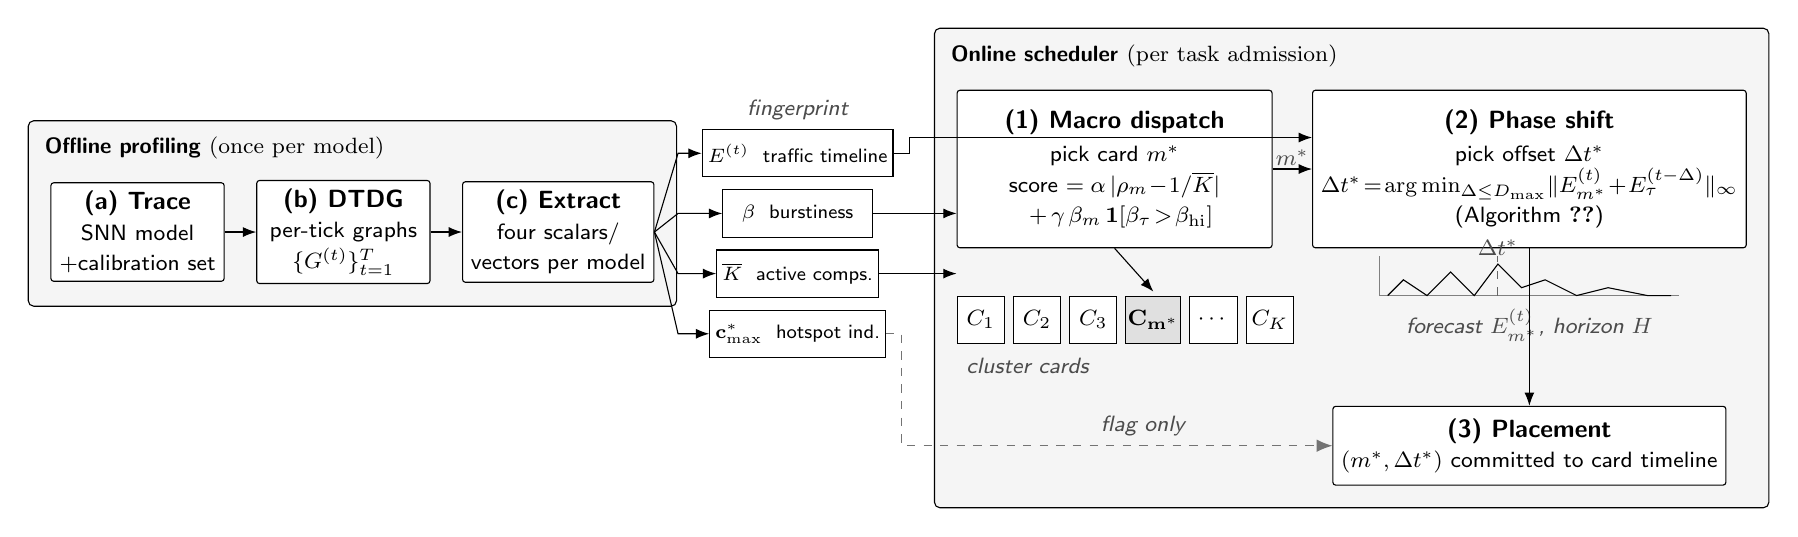
\begin{tikzpicture}[
        font=\sffamily\small,
        >={Latex[length=2mm,width=1.6mm]},
        node distance=0pt,
        proc/.style={draw,thin,rounded corners=1pt,align=center,inner sep=3pt,fill=white,
                     minimum width=22mm,minimum height=11mm},
        stage/.style={draw,thin,rounded corners=2pt,fill=black!4,inner sep=8pt},
        title/.style={font=\sffamily\bfseries\footnotesize,inner sep=2pt,fill=black!4},
        fp/.style={draw,thin,align=center,inner sep=2pt,fill=white,
                   font=\sffamily\scriptsize,minimum width=19mm,minimum height=6mm},
        card/.style={draw,thin,minimum width=7mm,minimum height=6mm,inner sep=0pt,
                     font=\sffamily\footnotesize,fill=white},
        lbl/.style={font=\sffamily\footnotesize\itshape,text=black!70},
        flow/.style={->,thin,>=Latex},
    ]

    % ====================================================================
    %  OFFLINE PROFILING  (three steps inside a labeled stage box)
    % ====================================================================
    \node[proc] (trace)   {\textbf{(a) Trace}\\\footnotesize SNN model\\\footnotesize +calibration set};
    \node[proc,right=4mm of trace] (dtdg) {\textbf{(b) DTDG}\\\footnotesize per-tick graphs\\\footnotesize $\{G^{(t)}\}_{t=1}^{T}$};
    \node[proc,right=4mm of dtdg] (extract) {\textbf{(c) Extract}\\\footnotesize four scalars/\\\footnotesize vectors per model};
	\draw[flow] (trace)   -- (dtdg);
	\draw[flow] (dtdg)    -- (extract);
	\coordinate (offline-title-pad) at ([yshift=5mm]trace.north west);

	\begin{scope}[on background layer]
	    \node[stage,fit=(offline-title-pad)(trace)(dtdg)(extract)] (offline) {};
	\end{scope}
    \node[title,anchor=north west] at ([xshift=4pt,yshift=-4pt]offline.north west)
        {Offline profiling \textnormal{\footnotesize(once per model)}};

    % ====================================================================
    %  FINGERPRINT BUS  (between offline and online)
    % ====================================================================
    \node[fp,right=6mm of extract.east,anchor=west,yshift=10mm] (Et)    {$E^{(t)}$~~traffic timeline};
    \node[fp,below=1.5mm of Et.south,anchor=north]               (beta)  {$\beta$~~burstiness};
    \node[fp,below=1.5mm of beta.south,anchor=north]             (Kbar)  {$\overline{K}$~~active comps.};
    \node[fp,below=1.5mm of Kbar.south,anchor=north]             (cstar) {$\mathbf{c}^{*}_{\max}$~~hotspot ind.};

    \coordinate (fpmid) at ($(extract.east)!0.5!(Et.west)$);
    \draw[flow] (extract.east) -- (fpmid |- Et)    -- (Et.west);
    \draw[flow] (extract.east) -- (fpmid |- beta)  -- (beta.west);
    \draw[flow] (extract.east) -- (fpmid |- Kbar)  -- (Kbar.west);
    \draw[flow] (extract.east) -- (fpmid |- cstar) -- (cstar.west);

    \node[lbl,above=0pt of Et.north] {fingerprint};

    % ====================================================================
    %  ONLINE SCHEDULER  (two steps + card row inside a labeled stage box)
    % ====================================================================
    \node[proc,right=8mm of Et.east,anchor=west,minimum width=40mm,minimum height=20mm,yshift=-2mm] (macro)
        {\textbf{(1) Macro dispatch}\\[1pt]
         \footnotesize pick card $m^{*}$\\
         \footnotesize score $=\alpha\,|\rho_m\!-\!1/\overline{K}|$\\
         \footnotesize $\;\;+\,\gamma\,\beta_m\,\mathbf{1}[\beta_\tau\!>\!\beta_{\mathrm{hi}}]$};

    \node[proc,right=5mm of macro.east,anchor=west,minimum width=40mm,minimum height=20mm] (phase)
        {\textbf{(2) Phase shift}\\[1pt]
         \footnotesize pick offset $\Delta t^{*}$\\
         \footnotesize $\Delta t^{*}\!=\!\arg\min_{\Delta\le D_{\max}}\!\|E^{(t)}_{m^{*}}\!+\!E^{(t-\Delta)}_{\tau}\|_\infty$\\
         \footnotesize (Algorithm~\ref{alg:phase_shift})};

    % card row beneath stage 1 — visualises candidate cards picked from
    \node[card,below=6mm of macro.south west,anchor=north west,minimum width=6mm] (c1) {$C_1$};
    \node[card,right=1mm of c1,minimum width=6mm] (c2) {$C_2$};
    \node[card,right=1mm of c2,minimum width=6mm] (c3) {$C_3$};
    \node[card,right=1mm of c3,fill=black!12,minimum width=7mm] (c4) {$\mathbf{C_{m^{*}}}$};
    \node[card,right=1mm of c4,minimum width=6mm] (c5) {$\cdots$};
    \node[card,right=1mm of c5,minimum width=6mm] (cK) {$C_K$};
    \node[lbl,below=0.5mm of c1.south west,anchor=north west] {cluster cards};
    \draw[flow] (macro.south) -- ($(c4.north)+(0,0.5mm)$);

    % forecast sparkline beneath stage 2 — visualises the timeline
    \begin{scope}[shift={($(phase.south)+(0,-6mm)$)}]
        \draw[thin,black!50] (-19mm,0) -- (19mm,0);
        \draw[thin,black!50] (-19mm,0) -- (-19mm,5mm);
        \draw[thin] (-18mm,0) -- (-16mm,2mm) -- (-13mm,0) -- (-10mm,3mm) -- (-7mm,0)
                 -- (-4mm,4mm) -- (-1mm,1mm) -- (2mm,2mm) -- (6mm,0) -- (10mm,1mm) -- (15mm,0) -- (18mm,0);
        % candidate offset marker
        \draw[thin,dashed,black!60] (-4mm,0) -- (-4mm,5mm);
        \node[lbl,anchor=south,inner sep=0pt] at (-4mm,5mm) {$\Delta t^{*}$};
        \node[lbl,anchor=north] at (0,-0.5mm) {forecast $E^{(t)}_{m^{*}}$, horizon $H$};
    \end{scope}

    % data flows into the online stages
    \draw[flow] (beta.east)  -- ++(2mm,0) |- (macro.west |- beta);
    \draw[flow] (Kbar.east)  -- ++(2mm,0) |- (macro.west |- Kbar);
    \draw[flow] (Et.east)    -- ++(2mm,0) |- ([yshift=4mm]phase.west);
    \draw[flow] (macro.east) -- node[lbl,above,inner sep=1pt]{$m^{*}$} (phase.west);

    % placement output
    \node[proc,below=20mm of phase.south,anchor=north,minimum width=40mm,minimum height=10mm]
        (place) {\textbf{(3) Placement}\\\footnotesize $(m^{*},\Delta t^{*})$ committed to card timeline};
    \draw[flow] (phase.south) -- ++(0,-3mm) -| (place.north);

	% hotspot indicator — currently recorded only
	\draw[->,thin,dashed,black!55] (cstar.east) -- ++(2mm,0) |- (place.west)
	    node[lbl,pos=0.78,above]{flag only};
	\coordinate (online-title-pad) at ([yshift=5mm]macro.north west);

	\begin{scope}[on background layer]
	    \node[stage,fit=(online-title-pad)(macro)(phase)(c1)(cK)(place)] (online) {};
	\end{scope}
    \node[title,anchor=north west] at ([xshift=4pt,yshift=-4pt]online.north west)
        {Online scheduler \textnormal{\footnotesize(per task admission)}};

    \end{tikzpicture}%
    }
    \caption{STPS pipeline. \emph{Offline:} a model is traced, lifted into a discrete-time dynamic graph, and reduced to four fingerprints. \emph{Online:} each admission runs in two stages --- macro-dispatch picks a card $m^{*}$ from $\{C_1,\dots,C_K\}$ using $\overline{K}$ and $\beta$, then phase-shift picks a start offset $\Delta t^{*}\!\le\!D_{\max}$ that fits the task's traffic timeline into a valley of the card's forecast. The hotspot indicator $\mathbf{c}^{*}_{\max}$ is recorded but does not drive placement in the current system (dashed arrow).}
    \label{fig:arch}
\end{figure*}

\subsection{Workload Fingerprint}
\label{sec:design:fingerprint}

We model an SNN inference as a Discrete-Time Dynamic Graph (DTDG) $\mathcal{G} = \{G^{(1)}, \dots, G^{(T)}\}$, where each snapshot $G^{(t)} = (\mathcal{V}, \mathcal{E}^{(t)}, W^{(t)})$ shares the same vertex set $\mathcal{V}$ of hardware-aligned neural populations (each population fits within one CIM core) and a per-tick weight tensor $W^{(t)}_{ij}$ measuring the expected spike traffic on edge $i\!\to\!j$. The expectation is taken over a calibration set drawn from the model's evaluation distribution, so the fingerprint is independent of any single input.

From this trace we extract three quantities that the online scheduler consumes:

\begin{itemize}
    \item \textbf{Traffic timeline $E^{(t)} \in \mathbb{R}^T$.} The total spike traffic at tick $t$, averaged over the calibration set. $E^{(t)}$ is the only fingerprint that retains temporal shape.
    \item \textbf{Global burstiness $\beta = \max_t E^{(t)} / \overline{E}$.} Peak-to-mean ratio of the traffic timeline; $\beta \approx 1$ for steady workloads, $\beta \gg 1$ for event-driven bursts.
    \item \textbf{Mean active components $\overline{K}$.} Mean number of connected components in the active-edge subgraph of $G^{(t)}$, averaged over $t$. $\overline{K}\!\to\!1$ indicates a topologically cohesive model; $\overline{K} \gg 1$ indicates several concurrent, weakly-coupled subflows.
\end{itemize}

A fourth quantity, the per-population maximum in-eigenvector centrality $\mathbf{c}^{*}_{\max}[i] = \max_t c^{(t)}_i$, is recorded as a hotspot indicator and discussed in Section~\ref{sec:design:spatial}.

The fingerprint is on the order of tens of kilobytes per model and is computed once at deployment time; subsequent scheduling decisions read it as a memory-mapped artefact.

\subsection{Online Scheduler}
\label{sec:design:online}

This subsection details the two stages summarised in Section~\ref{sec:design:overview}.

\subsubsection{Stage 1: Macro-Card Dispatch}
\label{sec:design:macro}

The cluster constraint we enforce is single-card placement: each model resides entirely on one card. The dispatch problem therefore reduces to selecting one card among those with sufficient free cores and memory for $\tau$. We score each feasible card $m$ by
\begin{equation}
    \mathcal{S}_m(\tau) \;=\; \alpha\,\bigl|\,\rho_m \,-\, \tfrac{1}{\overline{K}_\tau}\,\bigr| \;+\; \gamma\,\beta_m \cdot \mathbb{1}[\beta_\tau > \beta_{\text{hi}}],
    \label{eq:macro_score}
\end{equation}
where $\rho_m$ is the largest contiguous free-block ratio on card $m$ and $\beta_m$ is its running mean burstiness. The first term matches the task's topological cohesion against the card's available shape: cohesive tasks ($\overline{K}_\tau\!\to\!1$) are drawn to cards with large contiguous blocks ($\rho_m\!\to\!1$), while decoupled tasks ($\overline{K}_\tau \gg 1$) absorb fragmented cards without penalty. The second term keeps high-burstiness tasks away from cards that already host bursty workloads; it activates only above a threshold $\beta_{\text{hi}}$ so that flat traffic incurs no temporal penalty. The card with minimum $\mathcal{S}_m$ wins.

\subsubsection{Stage 2: Temporal Phase-Shifting}
\label{sec:phase_shift}

Cards co-locate multiple tasks, and their traffic timelines superpose on the same on-chip network. Spatial dispatch alone does not prevent two bursty tasks from peaking on the same tick. Stage~2 exploits the fact that the timeline $E_\tau^{(t)}$ is known at admission to delay $\tau$'s injection so that its peaks fall into the valleys of the existing card-level forecast.

Let $E_m^{(t)}$ be the forecasted background traffic on the selected card $m$ and $D_{\max}$ the deadline-bounded shift budget. The optimal offset is
\begin{equation}
    \Delta t^{*} \;=\; \arg\min_{\Delta t \in [0,\, D_{\max}]}\; \max_t\,\bigl(E_m^{(t)} + E_\tau^{(t - \Delta t)}\bigr),
    \label{eq:phase_shift}
\end{equation}
subject to the resulting peak staying below the per-card bandwidth ceiling $BW_{\max}$. When no offset in $[0, D_{\max}]$ satisfies the ceiling, the task is admitted unshifted (offset $0$) --- it is never dropped --- and simply contributes its share to congestion; we call this an \emph{offset-infeasible} admission, and it is rare except at extreme load. Algorithm~\ref{alg:phase_shift} expresses this as a single linear scan over $D_{\max}{+}1$ candidate offsets; the cost is $O(D_{\max} \cdot H)$ per task.

\begin{algorithm}[t]
\caption{Phase-Shift Selection}
\label{alg:phase_shift}
\begin{algorithmic}[1]
\Require Background $E_m$, task $E_\tau$, budget $D_{\max}$, ceiling $BW_{\max}$
\Ensure Offset $\Delta t^{*} \in [0, D_{\max}]$ (offset $0$ if none fits under $BW_{\max}$)
\State $p^* \gets \infty$,\; $\Delta t^{*} \gets 0$ \Comment{default: admit unshifted}
\For{$\Delta t = 0$ \textbf{to} $D_{\max}$}
    \State $p \gets \max_t \bigl(E_m^{(t)} + \mathrm{Shift}(E_\tau, \Delta t)^{(t)}\bigr)$
    \If{$p \le BW_{\max}$ \textbf{and} $p < p^*$}
        \State $p^* \gets p$,\; $\Delta t^{*} \gets \Delta t$
    \EndIf
\EndFor
\State $E_m \gets E_m + \mathrm{Shift}(E_\tau, \Delta t^{*})$
\State \Return $\Delta t^{*}$
\end{algorithmic}
\end{algorithm}

\subsection{Spatial Mapping and Hotspot Indicator}
\label{sec:design:spatial}

Once a card and offset are fixed, populations are mapped to PIM cores by the vendor compiler under standard hardware constraints. The fingerprint exposes $\mathbf{c}^{*}_{\max}$ as a per-population indicator of compute concentration: a population whose centrality exceeds a threshold $\theta_c$ is a candidate for splitting across adjacent cores, trading a small spatial footprint for reduced peak SOP pressure. In the current system this flag is recorded on the task but does not drive placement; we leave the centrality-driven splitting pass, and its end-to-end evaluation, to future work.

\subsection{Discussion}
\label{sec:design:discussion}

Two design choices warrant comment. First, all four fingerprint quantities are scalars or short vectors; the scheduler never inspects the underlying $T \times |\mathcal{V}|^2$ trace at runtime. This keeps admission cost independent of model size and is what allows STPS to interleave with arrival rates of thousands of tasks per second. Second, the macro-dispatch score in Equation~\ref{eq:macro_score} is deliberately a weighted sum rather than a lexicographic policy: the same scalar handles both empty and saturated regimes, so STPS degrades gracefully as cluster load increases rather than switching between policies.


\section{Implementation}
\label{sec:impl}

We implement STPS as a Python prototype on top of a discrete-event simulator of a multi-card CIM cluster. The system is partitioned into three packages so that the offline profiler, the online scheduler, and the simulation harness can evolve independently. The fingerprint extractor (\textsc{fingerprint/}, $\sim$2\,kLoC) lifts an SpikingJelly~\cite{fang2023spikingjelly} run into a DTDG and reduces it to the four quantities of Section~\ref{sec:design:fingerprint}; the resulting artefact is persisted as a memory-mapped \texttt{.npz} blob ($\sim$tens of kilobytes per model) and re-loaded lazily at admission time, so cold-start cost is a single file read. The online scheduler (\textsc{schedule/}, $\sim$0.8\,kLoC) implements both stages and a pluggable registry that exposes RR, BestFit, DRF, P2C, and the STPS variants behind a uniform interface; the registry also hosts the stage ablations as named entry points so the evaluation harness can sweep policies without touching the simulator core.

The simulation harness (\textsc{simulation/}, $\sim$0.5\,kLoC) implements the two-tier tick loop --- per-card placement, NoC bandwidth accounting, pending-traffic queue --- in pure NumPy; we deliberately avoid a hardware-cycle-accurate model because the scheduling decision is made entirely at admission, and the per-tick simulation only has to be accurate \emph{enough} to faithfully expose the bandwidth ceiling and queue dynamics. The whole system is around 4.6\,kLoC of Python and 1.8\,kLoC of pytest tests, exercised through a \texttt{Makefile} that drives both the per-policy runs and the cross-scheduler comparison sweeps used in Section~\ref{sec:eval}. The fingerprint extractor can also be invoked standalone (\texttt{python -m fingerprint.cli}) to produce synthetic fingerprints, which is what the steady-flat and pulse-train workloads in Section~\ref{sec:eval:setup} are built from.


\section{Evaluation}
\label{sec:eval}

The evaluation answers four questions. \textbf{RQ1} (Section~\ref{sec:eval:congestion}): does STPS reduce end-to-end NoC congestion, and at what cost? \textbf{RQ2} (Section~\ref{sec:eval:spatial}): do macro-dispatch and phase-shift attack congestion along complementary axes, so that neither stage alone suffices? \textbf{RQ3} (Section~\ref{sec:eval:temporal}): in which operating regimes does the relief hold, and where does it degrade? \textbf{RQ4} (Section~\ref{sec:eval:tail}): where in the delay distribution does STPS pay for the relief?

The headline finding is a worst-case one. At 16 cards STPS is the only scheduler that keeps the busiest card's NoC pressure below $13.5\times$ the cluster mean under every arrival process, while capacity-blind baselines let it climb to $24\times$ --- a $1.8\times$ reduction in the metric that determines when a card's NoC saturates first. It reaches that bound while \emph{preserving} cluster throughput to within 1--2\,\% and lowering mean congestion in all six cells tested, and it is the only baseline-competitive policy to win congestion in every cell rather than trading leadership. The costs are equally explicit and confined: STPS spends its entire delay penalty on the worst $\sim$1\,\% of tasks (Section~\ref{sec:eval:tail}) and does not improve across-card load dispersion --- that is a cost it pays for congestion relief, not a claim it makes.

\subsection{Trace-Driven Setup Exposes NoC Contention}
\label{sec:eval:setup}

\textbf{The simulator models per-card NoC pressure.} We use a discrete-event, trace-driven simulator of a multi-card CIM cluster (Section~\ref{sec:design}). Each card holds 256 cores wired by a 2D mesh NoC. The engine accounts for per-card instantaneous demand, NoC bandwidth cap $BW_{\max}$, and a pending-traffic queue that absorbs over-budget injection rather than dropping the task; the queue is drained at the cap rate so no task is ever rejected and the cluster's completion rate is always 1.0. All schedulers share the simulator and the same per-card placement primitive; they differ only in the admission-time dispatch and (for STPS) phase-shift logic.

\textbf{Workloads mix synthetic extremes with real SNN traces.} Each task draws a fingerprint from a \emph{mixed} set: four synthetic templates (steady-flat, two pulse trains with periods $T\!=\!8$ and $T\!=\!16$, and a heavy-tail burst) plus three real SpikingJelly~\cite{fang2023spikingjelly} traces (Spikformer~\cite{zhou2023spikformer}-CIFAR10, QKFormer-CIFAR10, SpikingResFormer-Tiny-ImageNet). Task arrivals follow either a Poisson process, a bursty arrival pattern that bunches admissions into onset windows, or a 1:1 mix of the two.

\textbf{Trace-derived NoC injection is the modeled bottleneck.} The simulator abstracts the cluster at the granularity our claims live at: per-card, per-tick NoC injection. Three properties make this sufficient to support the conclusions. First, the traffic timeline $E_\tau^{(t)}$ that drives every placement and phase-shift decision is \emph{trace-derived}, not parametric: the three real fingerprints are extracted from actual SpikingJelly spike tensors via the offline DTDG pipeline (Section~\ref{sec:design:fingerprint}), so the burst shapes the scheduler reacts to are the ones the models actually produce. The four synthetic templates exist only to sweep extremes (perfectly flat, single-period, heavy-tail) that the real traces sample but do not isolate. Second, the contended resource we model --- the NoC bandwidth cap and the pending-traffic queue draining at that cap --- is the resource SNN inference on CIM actually serialises on: with weights resident in memory, inference is communication- not compute-bound, so an injection-rate model captures the first-order bottleneck while remaining agnostic to per-core compute timing that scheduling does not influence. Third, the cap itself is not a tuned knob: $BW_{\max}$ is fixed at the p75 of the per-card demand observed under an \emph{uncapped} run, a workload-derived operating point at which every scheduler --- ours included --- sees congestion, rather than a value chosen to flatter STPS. We report the sensitivity of our conclusions to this choice across three cap-binding regimes in Section~\ref{sec:eval:temporal}.

\textbf{The methodology supports policy-level claims.} Three boundaries follow from a simulation-first study. First, the bandwidth cap is set from the workload itself (p75 of uncapped demand) rather than calibrated against a specific silicon NoC, whose effective cap depends on routing, arbitration, and contention that an injection-rate model abstracts away; we bracket this uncertainty with the cap-binding sweep of Appendix~\ref{app:regime}, whose binding, light, and non-binding regimes span the congestion levels a heavier (p50-like) or lighter (p90-like) cap would induce, and STPS's qualitative ordering holds across all three. Second, the fingerprints are extracted from the same calibration traces against which the scheduler is evaluated; a deployment trace that drifts from the calibration trace would erode Stage~A's topology score --- an effect RQ3 characterises along the predictability axis but does not isolate as an explicit calibration-to-deployment mismatch. Third, the numbers are throughput, congestion, and delay in a discrete-event model, not wall-clock latency on hardware; closing that gap requires a cycle-accurate or silicon NoC study we leave to future work. We therefore read our results as evidence about scheduling \emph{policy} under a faithful first-order NoC model, not as absolute performance predictions for a specific CIM part.

\textbf{The default configuration fixes a congested operating point.} Unless stated otherwise the cluster has $M\!=\!4$ cards, runs for 512 ticks, $BW_{\max}\!=\!9\!\times\!10^{5}$ (the p75 of the per-card demand observed under an uncapped run, so all schedulers see meaningful congestion), $D_{\max}\!=\!2$, $H\!=\!64$. We average each configuration over 5 seeds (21, 42, 99, 123, 2024) and report $\pm$95\,\% confidence half-widths where space permits; steady-state metrics skip the first and last 64 ticks of each run. The 16-card configuration scales the task count to 3200 to keep utilisation comparable.

\textbf{Baselines are fingerprint-blind spatial schedulers.} Round-robin (\textbf{RR}), best-fit on free cores (\textbf{BestFit}), dominant-resource fairness (\textbf{DRF})~\cite{ghodsi2011dominant}, and power-of-two-choices (\textbf{P2C})~\cite{mohan2022looking}. All four are spatial-only: they ignore fingerprints and inject tasks with zero offset. For the Stage-A ablation we isolate STPS's macro-dispatch as the spatial-only variant \textsc{stps-spatial}; for the Stage-B ablation we additionally pair each baseline with the phase-shift module (\textsc{+ps}). The full STPS scheduler is the \textsc{stps-spatial+ps} pairing.

\textbf{Metrics lead with congestion, then throughput, tail, and balance diagnostics.} The metrics that carry our claims are the congestion ones: (i) NoC \emph{congestion ratio} (the fraction of demand pushed back by the cap) and the mean wait in the pending queue (\emph{cong-wait}, ticks), and (ii) the max/min load ratio, which we read as \emph{worst-card NoC pressure} --- the busiest card's served load relative to the least-loaded, i.e.\ how far the hottest card runs ahead of the cluster. Alongside these we report (iii) cluster \emph{throughput} in tasks/tick and (iv) the p99 of per-task end-to-end delay, which we use to characterise the tail trade in Section~\ref{sec:eval:tail}. Finally, as \emph{diagnostics} --- not objectives STPS optimises --- we report the cross-card load coefficient of variation \emph{CV} and Jain's fairness index \emph{JFI}~\cite{jain1984quantitative} ($\mathrm{JFI}=(\sum_m L_m)^2/(M\sum_m L_m^2)\in(1/M,1]$, $1$ = perfectly balanced), together with the load-imbalance factor \emph{LIF} ($\mathrm{LIF}=\max_m L_m/\overline{L}\ge 1$); these measure across-card dispersion, which STPS does not target and on which it does not beat the baselines. To separate Stage-B's intrinsic offset from genuine queueing, we additionally report the \emph{cold-start-excluded throughput}, $N_{\text{completed}} / (T_{\text{steps}} - \overline{T_{\text{cold}}})$, where $\overline{T_{\text{cold}}}$ is the per-run mean start offset committed by phase-shift.

\subsection{RQ1: STPS Consistently Reduces NoC Congestion}
\label{sec:eval:congestion}

\begin{table*}[t]
\centering
\caption{End-to-end comparison on the mixed-fingerprint workload (5 seeds, mean values; bold = best in column within each cell). Among the four fingerprint-blind baselines, STPS is the \emph{only} scheduler that wins on both congestion metrics --- congestion ratio and mean queueing wait --- in every $\{$arrival, scale$\}$ cell, six out of six, at a 1--2\,\% throughput cost and a 6--20 tick increase in p99 tail delay. At 16 cards the same mechanism is the only one that keeps worst-card NoC pressure (max/min served load) under $13.5\times$ across all three arrivals, while every baseline exceeds $16\times$ --- and P2C reaches $23.9\times$ --- in at least one. The CV and JFI columns confirm the flip side of that trade: STPS runs the \emph{highest} across-card CV in every cell, so it does not improve --- and does not claim to improve --- load dispersion.}
\label{tab:q0_main}
\small
\setlength{\tabcolsep}{4pt}
\begin{tabular}{lllrrrrrrr}
\toprule
Scale & Arrival & Scheduler & CV $\downarrow$ & JFI $\uparrow$ & max/min $\downarrow$ & tput $\uparrow$ & cong. ratio $\downarrow$ & cong. wait $\downarrow$ & p99 $\downarrow$ \\
\midrule
\multirow{15}{*}{4 cards} & \multirow{5}{*}{Poisson}
   & RR       & \textbf{0.267} & \textbf{0.915} & \textbf{5.01} & \textbf{1.318} & 0.269          & 9.26          & \textbf{121.6} \\
 & & BestFit  & 0.288          & 0.904          & 9.05          & 1.303          & 0.260          & 9.06          & 137.4 \\
 & & DRF      & 0.288          & 0.904          & 9.05          & 1.303          & 0.260          & 9.06          & 137.4 \\
 & & P2C      & 0.275          & 0.912          & 5.45          & 1.314          & 0.265          & 9.13          & 130.0 \\
 & & \textbf{STPS}     & 0.293          & 0.903          & 5.46          & 1.292          & \textbf{0.247} & \textbf{8.42} & 141.4 \\
\cmidrule(l){2-10}
 & \multirow{5}{*}{Bursty}
   & RR       & 0.287          & \textbf{0.906} & 6.11          & 1.293          & 0.258          & 8.87          & 129.6 \\
 & & BestFit  & \textbf{0.286} & 0.904          & 6.06          & \textbf{1.296} & 0.258          & 8.89          & \textbf{127.2} \\
 & & DRF      & \textbf{0.286} & 0.904          & 6.06          & \textbf{1.296} & 0.258          & 8.89          & \textbf{127.2} \\
 & & P2C      & 0.294          & 0.901          & \textbf{5.80} & 1.286          & 0.255          & 8.86          & 135.2 \\
 & & \textbf{STPS}     & 0.307          & 0.896          & 6.23          & 1.269          & \textbf{0.239} & \textbf{8.14} & 143.4 \\
\cmidrule(l){2-10}
 & \multirow{5}{*}{Mixed}
   & RR       & \textbf{0.265} & \textbf{0.916} & 5.53          & \textbf{1.325} & 0.267          & 9.31          & \textbf{200.2} \\
 & & BestFit  & 0.292          & 0.902          & 6.19          & 1.309          & 0.259          & 9.21          & 212.0 \\
 & & DRF      & 0.292          & 0.902          & 6.19          & 1.309          & 0.259          & 9.21          & 212.0 \\
 & & P2C      & 0.275          & 0.911          & \textbf{5.16} & 1.316          & 0.263          & 9.25          & 207.0 \\
 & & \textbf{STPS}     & 0.300          & 0.898          & 6.24          & 1.297          & \textbf{0.245} & \textbf{8.56} & 215.4 \\
\midrule
\multirow{15}{*}{16 cards} & \multirow{5}{*}{Poisson}
   & RR       & 0.305          & 0.912          & 16.90         & \textbf{5.346} & 0.275          & 9.45          & 101.0 \\
 & & BestFit  & 0.307          & 0.911          & 21.52         & 5.321          & 0.274          & 9.41          & 104.6 \\
 & & DRF      & 0.307          & 0.911          & 21.52         & 5.321          & 0.274          & 9.41          & 104.6 \\
 & & P2C      & \textbf{0.303} & \textbf{0.913} & 21.78         & 5.339          & 0.276          & 9.53          & \textbf{98.0} \\
 & & \textbf{STPS}     & 0.317          & 0.906          & \textbf{13.42} & 5.274         & \textbf{0.256} & \textbf{8.61} & 107.2 \\
\cmidrule(l){2-10}
 & \multirow{5}{*}{Bursty}
   & RR       & 0.313          & 0.907          & 21.09         & 5.263          & 0.268          & 9.14          & 100.2 \\
 & & BestFit  & 0.318          & 0.904          & 14.62         & 5.251          & 0.267          & 9.12          & 100.8 \\
 & & DRF      & 0.318          & 0.904          & 14.62         & 5.251          & 0.267          & 9.12          & 100.8 \\
 & & P2C      & \textbf{0.311} & \textbf{0.908} & 23.90         & \textbf{5.279} & 0.271          & 9.25          & \textbf{97.2} \\
 & & \textbf{STPS}     & 0.325          & 0.901          & \textbf{12.09} & 5.212         & \textbf{0.252} & \textbf{8.45} & 105.4 \\
\cmidrule(l){2-10}
 & \multirow{5}{*}{Mixed}
   & RR       & \textbf{0.303} & \textbf{0.913} & 16.34         & \textbf{5.348} & 0.276          & 9.48          & 107.6 \\
 & & BestFit  & 0.307          & 0.910          & 13.45         & 5.337          & 0.274          & 9.49          & 110.2 \\
 & & DRF      & 0.307          & 0.910          & 13.45         & 5.337          & 0.274          & 9.49          & 110.2 \\
 & & P2C      & 0.304          & 0.912          & \textbf{12.20} & 5.346         & 0.275          & 9.50          & \textbf{107.0} \\
 & & \textbf{STPS}     & 0.316          & 0.906          & 12.80         & 5.289          & \textbf{0.257} & \textbf{8.62} & 114.2 \\
\bottomrule
\end{tabular}
\end{table*}

\paragraph{Congestion falls in every cell.} Table~\ref{tab:q0_main} reports STPS against the four baselines on the same workload at two cluster sizes. The primary result is in the congestion columns: STPS wins all six arrival/scale cells on both the congestion ratio and the mean queueing wait, and no baseline wins on either metric in any cell. The per-cell margin is small in absolute terms (5--7\,\% on the ratio, 7--9\,\% on the wait), but the contribution is the \emph{consistency}, not the magnitude: the baselines trade leadership from cell to cell, so an operator cannot pick one that is safe everywhere, whereas STPS is safe everywhere by construction. The wins are also statistically separated: every congestion-ratio and queue-wait improvement in Table~\ref{tab:q0_main} exceeds the combined 95\,\% confidence half-widths of STPS and the best baseline in its cell. The tightest margin --- 4-card bursty congestion ratio --- is $0.016$ against a combined half-width of $0.010$; every other cell separates more cleanly, and the 16-card cells separate by an order of magnitude relative to their half-widths. The magnitude of the effect grows with scale, and that is where the headline sits (below).

\paragraph{Congestion reduction costs 1--2\,\% throughput and does not buy dispersion.} STPS does not dominate the dispersion diagnostics, and this is by design rather than a shortcoming to explain away: across the cells tested its across-card CV is 4--13\,\% \emph{higher} than the best baseline while throughput is 1--2\,\% lower. Two distinct mechanisms produce the throughput gap. First, Stage~B injects a non-zero start offset whenever the forecast peak would collide with the card's existing schedule; this offset appears as the cold-start budget $\overline{T_{\text{cold}}}\!\approx\!1.0$ tick under $D_{\max}\!=\!2$ and accounts for $\sim$0.2\,\% of the throughput delta (excluding it from the throughput denominator closes only 0.16--0.17\,\% of the 1--2\,\% gap). The remaining 0.8--1.8\,\% is contention avoidance: when phase-shift defers a task into a residual valley, the card injects strictly less per tick, trading a fraction of average throughput for lower instantaneous congestion. The higher CV has the same root cause: STPS chooses cards by topology fit and de-synchronises bursts in time rather than equalising instantaneous served load, so across-card variance rises even as the busiest card's absolute pressure falls (see below). Dispersion is simply not the axis STPS optimises.

\paragraph{STPS bounds worst-card NoC pressure at 16 cards.} The max/min column measures worst-card NoC pressure --- how far the busiest card runs ahead of the least-loaded --- and the effect it captures only emerges at scale. At 4 cards, where there are few placement choices, STPS sits marginally above the best baseline (e.g.\ 5.46 vs RR's 5.01 under Poisson), which is expected: with so few cards there is little room to steer the hottest one down, and STPS is optimising congestion, not dispersion. At 16 cards the picture changes: STPS is the only scheduler whose worst-card ratio stays under $13.5\times$ across all three arrivals ($13.4$/$12.1$/$12.8$), whereas every baseline exceeds $16\times$ in at least one arrival and P2C reaches $23.9\times$ under bursty load. The capacity policies that look evenly packed by core count develop the hottest cards exactly where the cluster has the most placement decisions to make; STPS's fingerprint-aware dispatch keeps the busiest card bounded. This reads as a congestion result, not a balance one: a card whose max/min runs to $24\times$ is a card whose NoC is saturating, and it is that saturation --- not the dispersion statistic --- that STPS suppresses. It is consistent with the design intent of Section~\ref{sec:design:macro}: the macro-dispatch score becomes more selective as more cards are available to score against, so the topology signal it carries scales with cluster size in a way capacity-only policies cannot match.

\begin{table}[t]
\centering
\caption{Throughput decomposition at 16 cards: cold-start-excluded throughput closes only $0.16$--$0.17$\,\% of the $1.3$--$1.4$\,\% gap to the best baseline. The remaining gap is contention-avoidance --- the price STPS pays to keep the NoC under its cap.}
\label{tab:q0_cold}
\small
\begin{tabular}{llrrr}
\toprule
Arrival & Scheduler & $\overline{T_{\text{cold}}}$ & tput & tput$_{\text{excl. cs}}$ \\
\midrule
\multirow{2}{*}{Poisson} & best baseline (RR) & 0.00 & 5.346 & 5.346 \\
                        & STPS               & 1.02 & 5.274 & 5.282 \\
\midrule
\multirow{2}{*}{Bursty}  & best baseline (P2C) & 0.00 & 5.279 & 5.279 \\
                        & STPS               & 1.01 & 5.212 & 5.221 \\
\bottomrule
\end{tabular}
\end{table}

\paragraph{The trade-off matches CIM contention.} Read as a whole, RQ1 is a "win the worst case at preserved cost" result. STPS does not chase average load balance; it targets the contention metric that dominates this CIM substrate --- the per-card NoC (Section~\ref{sec:bg:hardware}) --- and holds cluster throughput within 1--2\,\% of the best baseline while doing so. The payoff is concentrated where it matters: at scale it bounds worst-card NoC pressure below $13.5\times$ instead of the $24\times$ that P2C reaches, and a card running at $24\times$ the cluster mean is a card whose NoC saturates first and stalls its tenants. Buying a large reduction in that worst-case pressure for a throughput cost that stays in the noise is the operating point STPS is designed to serve.

\subsection{RQ2: Macro-Dispatch and Phase-Shift Are Complementary}
\label{sec:eval:spatial}

STPS combines macro-card dispatch with phase-shift scheduling, so the evaluation must isolate the contribution of each stage. Table~\ref{tab:q2_phase} holds the default congested operating point of Table~\ref{tab:q0_main} ($BW_{\max}\!=\!9\!\times\!10^{5}$, $D_{\max}\!=\!2$, 800 tasks, 4 cards) and decomposes each policy family into three variants: the spatial policy alone (\textsc{base}), the same policy augmented with phase-shift (\textsc{+ps}), and \textsc{stps-spatial} --- our macro-dispatch in isolation --- with and without phase-shift. The \textsc{stps-spatial+ps} row is the full scheduler. Comparing each \textsc{base} row with its \textsc{+ps} counterpart isolates Stage~B's marginal effect; comparing the spatial-only rows isolates Stage~A's placement effect. Stage~B is policy-agnostic by construction: it consumes the traffic timeline $E^{(t)}$ and the card forecast, scans up to $D_{\max}$ offsets, and commits the one whose forecast peak is lowest under the cap (Algorithm~\ref{alg:phase_shift}), so it can be attached to any spatial policy. The decomposition makes one thing immediate: bolting phase-shift onto a capacity baseline does drive congestion to zero, but it pays for that with a steep throughput loss \emph{and} a higher CV --- it is not a free win on any axis. Only the full STPS pairing relieves congestion at negligible throughput cost.

\begin{table*}[t]
\centering
\caption{Stage decomposition at the default congested workpoint (4 cards, mixed fingerprints, $BW_{\max}\!=\!9\!\times\!10^{5}$, $D_{\max}\!=\!2$, 800 tasks, 5 seeds): each spatial policy (\textsc{base}) paired with phase-shift (\textsc{+ps}), and STPS's own macro-dispatch \textsc{stps-spatial} with phase-shift added; the full scheduler is \textsc{stps-spatial+ps}. Attaching phase-shift to a capacity baseline drives the congestion ratio ($\sim$0.26) to zero, but the price is steep: throughput drops 15--21\,\% and CV \emph{rises} (RR $0.267\!\to\!0.313$, P2C $0.275\!\to\!0.532$), because de-synchronising bursts under a binding cap spreads served load less evenly, not more. Full STPS is the exception: it lowers congestion ($0.263\!\to\!0.247$) at essentially no throughput cost ($1.311\!\to\!1.292$) and only a modest CV rise, because Stage~A has already placed the load and Stage~B has little left to defer. Read each row as a full metric vector, not a single column.}
\label{tab:q2_phase}
\small
\begin{tabular}{llrrrrrr}
\toprule
Arrival & Policy & CV & throughput & cong.\ ratio & cong.\ wait & p99 delay & mean offset \\
\midrule
\multirow{10}{*}{Poisson}
 & RR \textsc{base}             & \textbf{0.267} & \textbf{1.318} & 0.269 & 9.26 & 121.6 & 0.00 \\
 & RR \textsc{+ps}              & 0.313          & 1.094 & \textbf{0.000} & \textbf{0.00} & \textbf{17.0} & 1.05 \\
 & BestFit \textsc{base}        & 0.288          & 1.303 & 0.260 & 9.06 & 137.4 & 0.00 \\
 & BestFit \textsc{+ps}         & 0.321          & 1.149 & 0.000 & 0.00 & 17.0 & 0.98 \\
 & P2C \textsc{base}            & 0.275          & 1.314 & 0.265 & 9.13 & 130.0 & 0.00 \\
 & P2C \textsc{+ps}             & 0.532          & 1.079 & 0.000 & 0.01 & 17.0 & 1.03 \\
 & \textsc{stps-spatial}        & 0.268          & 1.311 & 0.263 & 8.96 & 132.6 & 0.00 \\
 & \textbf{stps-spatial+ps}     & 0.293          & 1.292 & 0.247 & 8.42 & 141.4 & 0.99 \\
\midrule
\multirow{10}{*}{Bursty}
 & RR \textsc{base}             & \textbf{0.287} & 1.293 & 0.257 & 8.87 & 129.6 & 0.00 \\
 & RR \textsc{+ps}              & 0.393          & 1.041 & \textbf{0.000} & \textbf{0.00} & \textbf{17.0} & 0.95 \\
 & BestFit \textsc{base}        & \textbf{0.287} & \textbf{1.296} & 0.258 & 8.89 & 127.2 & 0.00 \\
 & BestFit \textsc{+ps}         & 0.408          & 1.076 & 0.000 & 0.01 & 17.0 & 0.89 \\
 & P2C \textsc{base}            & 0.294          & 1.286 & 0.255 & 8.86 & 135.2 & 0.00 \\
 & P2C \textsc{+ps}             & 0.600          & 1.015 & 0.000 & 0.01 & 17.0 & 0.98 \\
 & \textsc{stps-spatial}        & 0.277          & 1.303 & 0.260 & 8.81 & 121.8 & 0.00 \\
 & \textbf{stps-spatial+ps}     & 0.307          & 1.269 & 0.239 & 8.14 & 143.4 & 0.99 \\
\bottomrule
\end{tabular}
\end{table*}

\paragraph{Phase-shift zeroes congestion but pays in throughput.} Table~\ref{tab:q2_phase} reports the ablation. At the default congested workpoint the baseline congestion ratio is substantial ($\sim$0.26, queue wait $\sim$9 ticks); attaching phase-shift to RR, BestFit, DRF, or P2C drives it to exactly zero and empties the queue. The mechanism is direct: by deferring each task's onset by at most $D_{\max}\!=\!2$ ticks the optimiser finds a slot whose superposition on the card forecast stays below $BW_{\max}$. But the relief is bought with throughput. Tasks that cannot find a sub-cap slot are held back, and the steady-state window clips the deferred onsets, so throughput drops 15--21\,\% (RR Poisson $1.318\!\to\!1.094$, P2C bursty $1.286\!\to\!1.015$). \textsc{stps-spatial+ps} (full STPS) is the exception that proves the point: it lowers congestion from $0.263$ to $0.247$ while holding throughput at $1.292$ --- within $1.5$\,\% of its base --- because Stage~A has already spread the load spatially, leaving little for Stage~B to defer and few tasks to hold back.

\paragraph{Phase-shift raises CV under a binding cap.} The dispersion column tells the honest counterpart to the congestion win: at this congested workpoint phase-shift \emph{raises} CV for every spatial policy --- RR (Poisson $0.267\!\to\!0.313$), BestFit ($0.288\!\to\!0.321$), P2C ($0.275\!\to\!0.532$), and full STPS ($0.268\!\to\!0.293$). The mechanism is the flip side of congestion relief: when the cap binds, the baselines are already flattened to a low CV ($\approx$0.27) by the queue clipping their peaks uniformly, so any offset that de-synchronises bursts in time pulls served load off that flat profile and \emph{increases} across-card variance. P2C inflates most ($0.275\!\to\!0.532$) because its power-of-two base leaves the least temporal structure for the offset to work with, so the offsets scatter load furthest. This is not a defect to hide: it is direct evidence that phase-shift trades dispersion for congestion, and that dispersion is not the axis on which STPS competes. Appendix~\ref{app:regime} shows the sign reverses only when the cap is loose enough that the baselines retain their natural dispersion.

\paragraph{The two stages occupy complementary roles.} The decomposition makes the division of labour legible. Phase-shift on a capacity baseline drives congestion to exactly zero but at a steep 15--21\,\% throughput cost and a higher CV; macro-dispatch alone (\textsc{stps-spatial}) holds CV and throughput at the baseline but leaves most of the congestion ($\sim$0.26) in place. Only the pairing reaches a deployable compromise: full STPS is the single variant that lowers congestion ($0.263\!\to\!0.247$) while keeping throughput essentially flat ($1.311\!\to\!1.292$), whereas every baseline+phase-shift row that zeroes congestion sacrifices roughly a fifth of throughput to do it. Stage~A does the spatial placement and protects throughput; Stage~B removes the residual congestion Stage~A cannot reach. Their interaction is what makes STPS a scheduler rather than either stage alone: Stage~A leaves so little congestion that Stage~B need barely defer anything, so the throughput and dispersion penalties that cripple baseline+phase-shift never materialise. Table~\ref{tab:q2_phase} should therefore be read by its full metric vector --- congestion, CV, tail delay, and throughput together --- not a single column: a policy that zeroes congestion by giving up a fifth of throughput and inflating CV is not the operating point STPS targets.

\subsection{RQ3: STPS Helps in Predictable, Non-Extreme Regimes}
\label{sec:eval:temporal}

STPS is not designed to dominate every metric in every operating regime. This section maps the boundary explicitly along three axes an operator controls: how predictable the workload's topology is (does Stage~A's score carry signal?), how hard the bandwidth cap binds (is there congestion for Stage~B to lever?), and how large the offset budget $D_{\max}$ is (how much tail may phase-shift spend?). The main result is that STPS's two stages are \emph{conditional} levers: each helps in the regime it was designed for and degrades gracefully outside it, and the relevant conditions are observable before deployment.

\paragraph{Stage~A needs predictable fingerprints.} Stage~A consumes only two fingerprint quantities --- the topological cohesion $\overline{K}_\tau$ and the burstiness $\beta_\tau$ --- and emits a single scalar score. The question is: when does that score buy anything? We answer with two sweeps. The first varies cluster \emph{utilisation} on a single workload mix; the second varies the \emph{fingerprint composition} of the workload at fixed utilisation. Both are run on a 4-card cluster with 512 cores per card so that Stage~A is exercised in isolation (without $BW_{\max}$ binding and without Stage~B influence). All numbers below are 5-seed means; we report $\pm95$\,\% half-widths where they affect interpretation.

\begin{figure}[t]
\centering
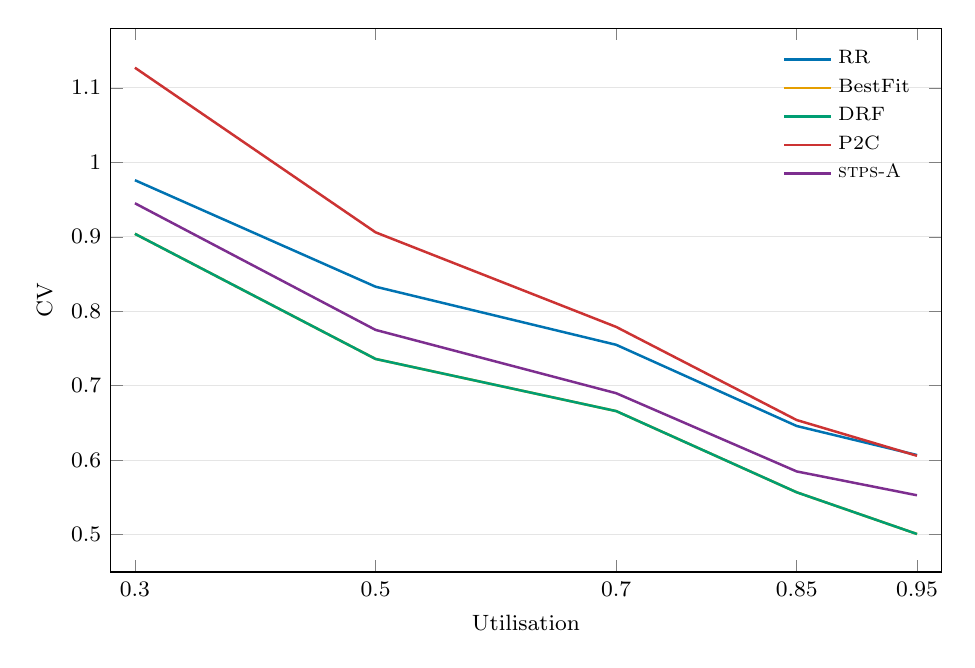
\begin{tikzpicture}
\begin{axis}[
    width=\linewidth,
    height=0.70\linewidth,
    xlabel={Utilisation},
    ylabel={CV},
    xmin=0.28, xmax=0.97,
    ymin=0.45, ymax=1.18,
    xtick={0.30,0.50,0.70,0.85,0.95},
    ymajorgrids=true,
    grid style={black!10},
    tick label style={font=\footnotesize},
    label style={font=\footnotesize},
    legend style={font=\scriptsize,draw=none,fill=none,at={(0.98,0.98)},anchor=north east},
    legend cell align={left},
    every axis plot/.append style={line width=0.9pt},
]
\addplot[algRR,solid,no markers] coordinates {(0.30,0.976) (0.50,0.833) (0.70,0.755) (0.85,0.646) (0.95,0.607)};
\addlegendentry{RR}
\addplot[algBestFit,solid,no markers] coordinates {(0.30,0.904) (0.50,0.736) (0.70,0.666) (0.85,0.557) (0.95,0.501)};
\addlegendentry{BestFit}
\addplot[algDRF,solid,no markers] coordinates {(0.30,0.904) (0.50,0.736) (0.70,0.666) (0.85,0.557) (0.95,0.501)};
\addlegendentry{DRF}
\addplot[algP2C,solid,no markers] coordinates {(0.30,1.127) (0.50,0.906) (0.70,0.779) (0.85,0.654) (0.95,0.606)};
\addlegendentry{P2C}
\addplot[algSTPS,solid,no markers] coordinates {(0.30,0.945) (0.50,0.775) (0.70,0.690) (0.85,0.585) (0.95,0.553)};
\addlegendentry{\textsc{stps-A}}
\end{axis}
\end{tikzpicture}
\caption{Stage~A under a utilisation sweep (4 cards $\times$ 512 cores, Poisson, mixed fingerprints, 5 seeds). Each point reports CV, so lower is better. Across the whole sweep BestFit/DRF hold the lowest CV because empty-capacity signals are the strongest placement cue; Stage~A tracks just above them (within $\sim$4--10\,\%) and stays ahead of RR and P2C. Dispersion falls monotonically as utilisation rises, but no policy --- Stage~A included --- reduces it below the capacity baselines: Stage~A is not a dispersion-minimising placement.}
\label{fig:q1_util}
\end{figure}

\paragraph{Utilisation determines whether topology matters.} Figure~\ref{fig:q1_util} plots CV, so lower values indicate more even load across cards. Two things are visible. First, BestFit and DRF lead at every utilisation: with cards distinguished mainly by free capacity, the capacity signal is the better placement cue and the $\overline{K}_\tau$-aware score cannot beat it on dispersion. Second, Stage~A nonetheless tracks the leaders closely --- within $\sim$4--10\,\% of BestFit and consistently ahead of RR and P2C --- and the whole field compresses as load rises and spatial freedom shrinks. The reading is not that Stage~A wins dispersion (it does not) but that it stays competitive on dispersion while buying the congestion relief that motivates it; topology-aware placement neither helps nor hurts balance materially in this regime.

\begin{figure}[t]
\centering
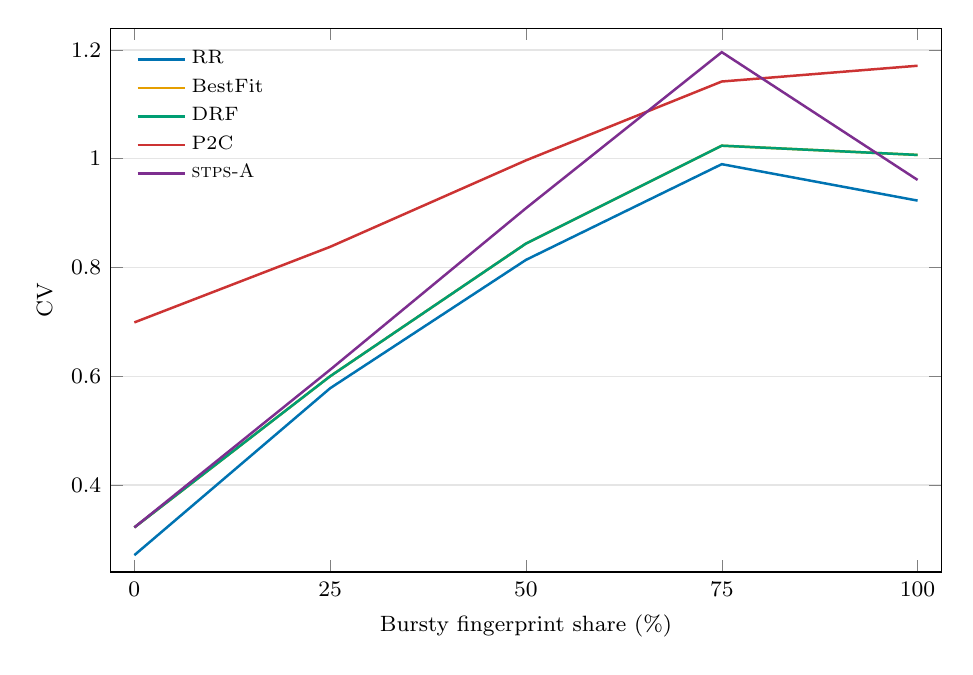
\begin{tikzpicture}
\begin{axis}[
    width=\linewidth,
    height=0.70\linewidth,
    xlabel={Bursty fingerprint share (\%)},
    ylabel={CV},
    xmin=-3, xmax=103,
    ymin=0.24, ymax=1.24,
    xtick={0,25,50,75,100},
    ymajorgrids=true,
    grid style={black!10},
    tick label style={font=\footnotesize},
    label style={font=\footnotesize},
    legend style={font=\scriptsize,draw=none,fill=none,at={(0.02,0.98)},anchor=north west},
    legend cell align={left},
    every axis plot/.append style={line width=0.9pt},
]
\addplot[algRR,solid,no markers] coordinates {(0,0.271) (25,0.578) (50,0.814) (75,0.990) (100,0.923)};
\addlegendentry{RR}
\addplot[algBestFit,solid,no markers] coordinates {(0,0.322) (25,0.600) (50,0.844) (75,1.024) (100,1.007)};
\addlegendentry{BestFit}
\addplot[algDRF,solid,no markers] coordinates {(0,0.322) (25,0.600) (50,0.844) (75,1.024) (100,1.007)};
\addlegendentry{DRF}
\addplot[algP2C,solid,no markers] coordinates {(0,0.699) (25,0.838) (50,0.997) (75,1.142) (100,1.171)};
\addlegendentry{P2C}
\addplot[algSTPS,solid,no markers] coordinates {(0,0.322) (25,0.612) (50,0.909) (75,1.196) (100,0.961)};
\addlegendentry{\textsc{stps-A}}
\end{axis}
\end{tikzpicture}
\caption{Stage~A under a fingerprint-composition sweep (4 cards, Poisson, 70\,\% utilisation). Each point reports CV, so lower is better; the x-axis gives the bursty share of a steady-flat/bursty mix. CV climbs with burstiness for every policy, because bursty fingerprints inject sharper per-card peaks that no placement can equalise. Stage~A tracks BestFit/DRF across the whole sweep --- tied at $0\,\%$ bursty and within the baseline band throughout --- so topology-aware placement neither wins nor loses dispersion as burstiness grows. RR happens to hold the lowest CV at the flat end; the fingerprint's value is congestion relief, not dispersion, which this sweep does not measure.}
\label{fig:q1_mix}
\end{figure}

\paragraph{Fingerprint composition does not make Stage~A a dispersion winner.} Figure~\ref{fig:q1_mix} fixes utilisation at 70\,\% and varies the workload from purely steady-flat to purely bursty fingerprints. CV rises with the bursty share for all five policies: sharper peaks are harder to spread, independent of the placement rule. Stage~A sits inside the baseline band the whole way --- tied with BestFit/DRF at $0\,\%$ bursty ($0.322$) and never separating by more than the baselines separate from each other --- so the fingerprint neither buys nor costs dispersion here. This matters for honesty about the design: Stage~A is a congestion lever, and its topology score does not translate into a load-dispersion advantage even in the steady-flat regime where the fingerprint is most predictable. The predictability the fingerprint provides pays off in where bursts land on the timeline (Stage~B, next), not in equalising served load across cards. It is exactly the bursty regime that Stage~B, analysed next, is built for --- the two stages cover complementary halves of the predictability axis.

\paragraph{Stage~B works best before hard saturation.} Phase-shift only relieves congestion where the cap binds. Sweeping the cap across three regimes --- binding ($BW_{\max}\!=\!9\!\times\!10^{5}$, 800 tasks; $\sim$0.26 baseline congestion), non-binding ($5\!\times\!10^{6}$, demand never reaches the cap), and lightly binding ($9\!\times\!10^{5}$, 400 tasks; $\sim$0.09) --- the congestion ratio drops to zero wherever there is congestion to remove (binding and light) and is undefined where there is none (non-binding). Its effect on dispersion has the opposite sign in the two congested regimes: under the hard-binding cap phase-shift \emph{raises} CV for every policy (the queue has already flattened the baselines, so any offset scatters load off that flat profile), whereas under the light cap it \emph{lowers} CV (the baselines keep enough natural dispersion that de-synchronising bursts helps). Either way the price is throughput (18--23\,\% binding, 14--16\,\% light) and tail (p99 rises everywhere, since the queue keeps baseline p99 at its $\sim$15-tick floor). The practical reading: STPS's sweet-spot is a correctly- or over-provisioned cluster, and full STPS ships $D_{\max}\!=\!2$ so the offset stays small; pushed into heavy congestion, the right response is provisioning, not a larger offset budget. Appendix~\ref{app:regime} gives the full per-policy grid and the sign structure of the CV effect.

\begin{table}[t]
\centering
\caption{How each metric responds as the phase-shift budget $D_{\max}$ grows from 2 to 16 (light regime C, 4 cards, mixed fingerprints, 5 seeds). Congestion --- the metric STPS targets --- is a switch, not a knob: it is already zeroed at $D_{\max}\!=\!2$. The dispersion diagnostics (CV/JFI/LIF, max/min) do improve with a larger budget in this loosely-capped regime, but with diminishing returns that saturate near $D_{\max}\!=\!8$, while tail delay and throughput cost grow monotonically. The columns pull in opposite directions, which is what fixes a small default.}
\label{tab:q2_dmax}
\small
\begin{tabular}{lll}
\toprule
Metric & Response to $D_{\max}\!\uparrow$ & Detail \\
\midrule
Cong.\ ratio (non-STPS) & flat at 0 from $D_{\max}\!=\!2$ & switch, not knob \\
Cong.\ ratio (STPS)     & slow $\downarrow$ & $0.087\!\to\!0.079$ \\
CV / JFI / LIF      & $\downarrow$, saturating & knee near $D_{\max}\!=\!8$ \\
Max/min                  & $\downarrow$ & $8$--$13 \to 3$--$6$ \\
p99 / mean offset        & $\uparrow$ monotone & offset $0.5\!\to\!4$ ticks \\
Throughput               & partial recovery & stays below baseline \\
\bottomrule
\end{tabular}
\end{table}

\paragraph{A small offset budget captures most of the gain.} A budget sweep $D_{\max} \in \{2,4,8,16\}$ at the light cap (Table~\ref{tab:q2_dmax}) shows the metric groups pulling against each other, with congestion the one that matters. Congestion relief is binary: the moment phase-shift is enabled, every capacity baseline's congestion ratio drops from $\sim$0.09 to zero, and no larger budget improves on zero. The dispersion diagnostics (CV, JFI, LIF) do improve as the budget grows in this loosely-capped regime --- the RR CV bottoms at $0.44$ for $D_{\max}\!=\!8$ then rebounds at $16$ --- but this is a side-effect, not the objective, and it saturates quickly. Tail delay moves the opposite way: the mean injected offset grows from $\sim$0.5 to $\sim$4 ticks across the sweep, dragging p99 up monotonically and clawing back the throughput that the cap rejections cost. The budget that buys the congestion switch while paying the least tail and throughput is the smallest one. We adopt $D_{\max}\!=\!2$ as the default: it already zeroes congestion, recovers the bulk of the worst-card-pressure compression ($8$--$13\times \to 3$--$6\times$), and holds the mean offset under one tick. On full STPS the case is sharper still --- a larger budget yields no congestion gain (Stage~A has already consumed the spatial slack) and only inflates p99, so $D_{\max}\!=\!2$ is strictly preferred. The cap-binding sweep (Appendix~\ref{app:regime}) explains which of these signals would persist or invert under a heavier cap, even at this attenuated budget.



\subsection{RQ4: Tail Delay Is Confined to the Worst 1\%}
\label{sec:eval:tail}

\begin{figure*}[t]
    \centering
    \begin{minipage}{0.48\linewidth}
        \centering
        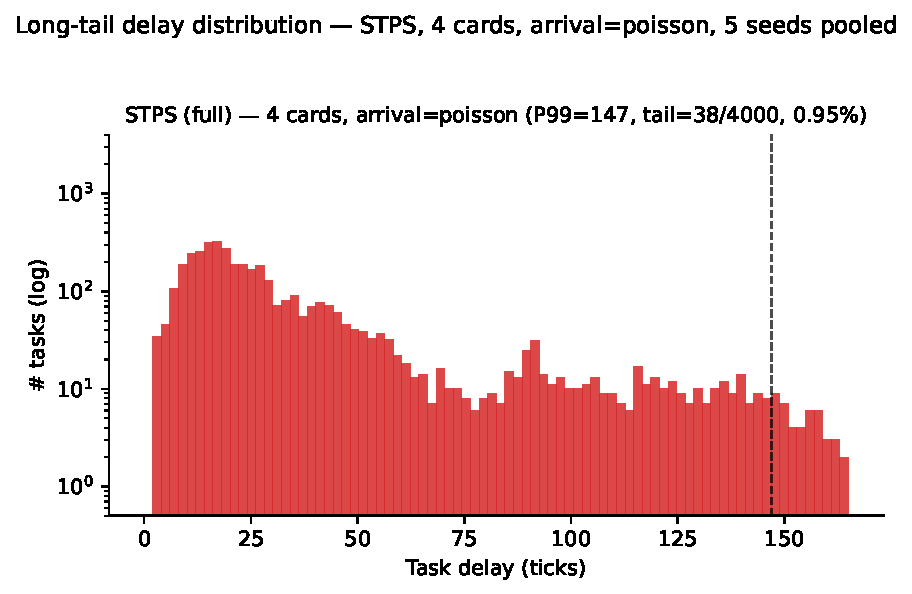
\includegraphics[width=\linewidth]{picture/stps_long_tail_4card_poisson.pdf}
        \\\footnotesize (a) 4 cards, Poisson
    \end{minipage}\hfill
    \begin{minipage}{0.48\linewidth}
        \centering
        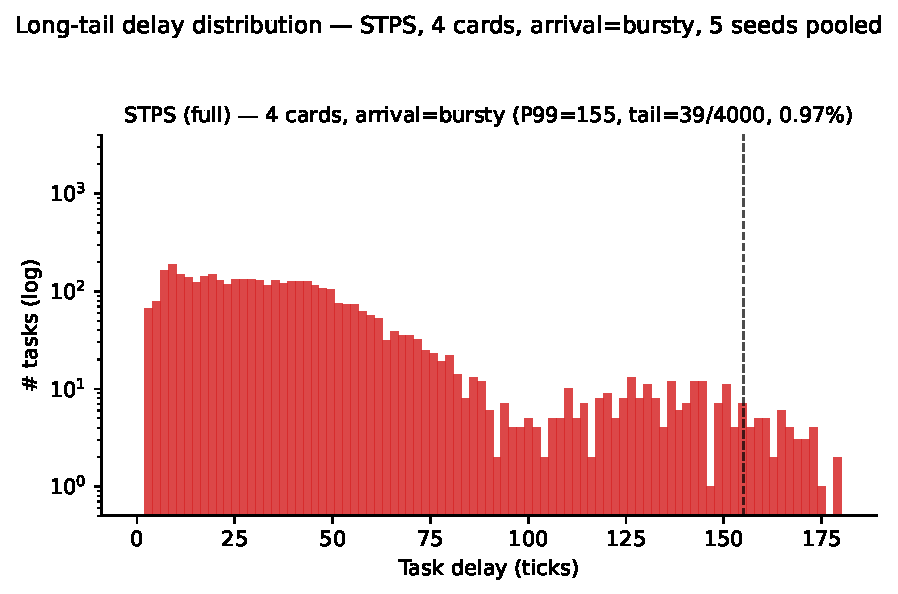
\includegraphics[width=\linewidth]{picture/stps_long_tail_4card_bursty.pdf}
        \\\footnotesize (b) 4 cards, Bursty
    \end{minipage}

    \vspace{0.6em}

    \begin{minipage}{0.48\linewidth}
        \centering
        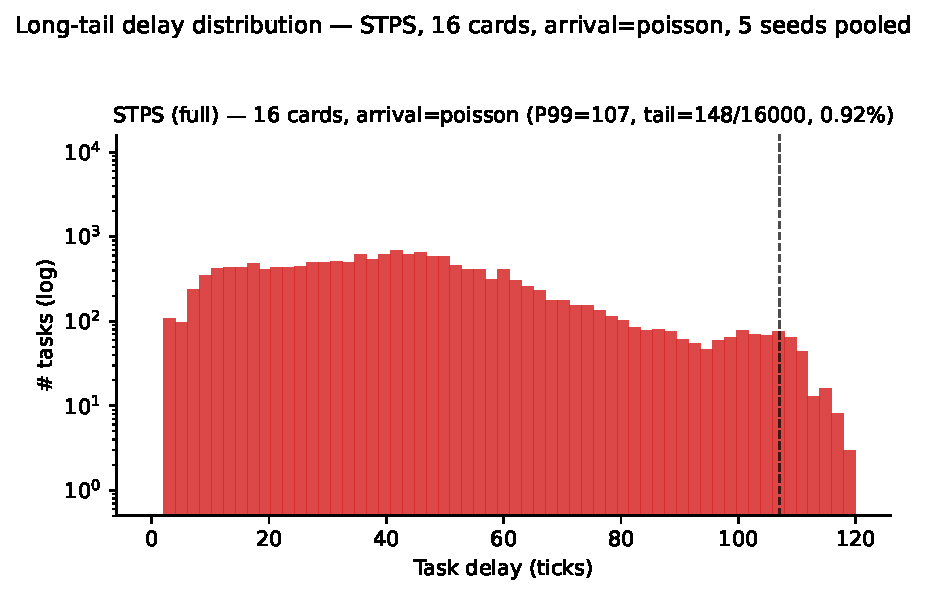
\includegraphics[width=\linewidth]{picture/stps_long_tail_16card_poisson.pdf}
        \\\footnotesize (c) 16 cards, Poisson
    \end{minipage}\hfill
    \begin{minipage}{0.48\linewidth}
        \centering
        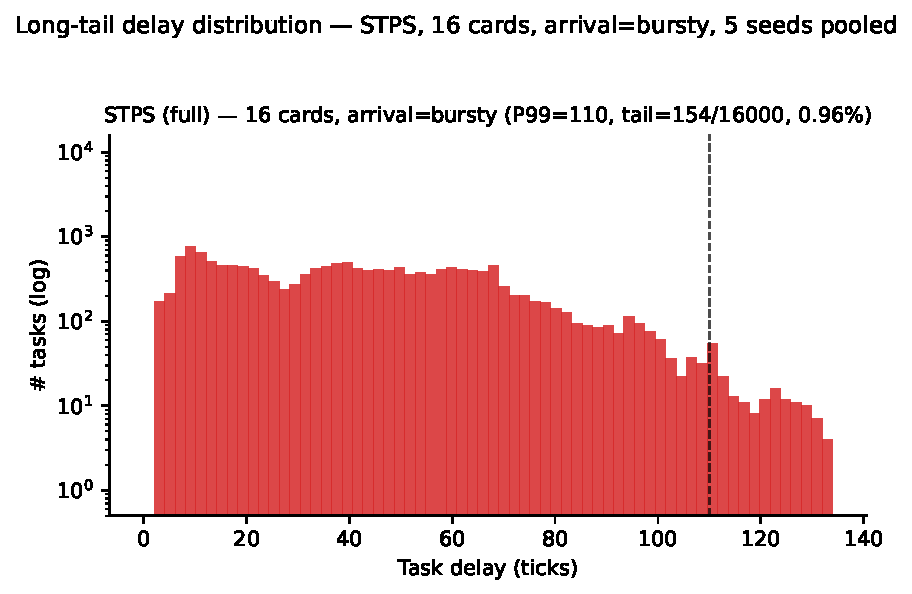
\includegraphics[width=\linewidth]{picture/stps_long_tail_16card_bursty.pdf}
        \\\footnotesize (d) 16 cards, Bursty
    \end{minipage}
    \caption{Delay survival functions across both cluster sizes and both arrival modes (5 seeds pooled, log--log). All schedulers track each other up to roughly the 90th percentile; STPS's curve only departs from the baselines above $\Pr[\text{delay}\!>\!d]\!\approx\!10^{-2}$. The tasks living in that upper-right corner --- the ones STPS finishes later --- are the same bursty, high-$\beta_\tau$ population that drives p99: STPS pays its tail price exclusively on the long-tail tasks, and pays it to buy the cluster-wide congestion relief and worst-card-pressure reduction documented in Table~\ref{tab:q0_main}.}
    \label{fig:longtail}
\end{figure*}

Averages flatter cluster schedulers. A scheduler that improves the median can still fail an SLA at the tail, and the tail is exactly where STPS's trade-off lives. Figure~\ref{fig:longtail} plots $\Pr[\text{delay}>d]$ for both the 4-card and 16-card clusters under both arrival modes; we show the two extreme arrival processes, omitting the Mixed panels because, as a 1:1 blend of Poisson and bursty, their survival curves lie between the two extremes and reveal no additional shape. The four panels tell a consistent story: up to roughly the 90th percentile every scheduler tracks every other within a few ticks; the curves only fan out in the upper-right corner. By construction, the tasks that populate that corner are the long-tail tasks --- the same bursty, high-$\beta_\tau$ population that defines p99 in the first place --- and STPS's slower-decaying curve sits to the right of the baselines precisely on those tasks. At p99 on 16 cards STPS trails the best baseline by 6--9 ticks (e.g.\ 107 vs 98 under Poisson, 105 vs 97 under bursty); the 4-card panels show the same shape at a larger absolute tail price ($\sim$15--20 ticks). Crucially, the curves are indistinguishable on the body: STPS does not slow median or p90 tasks; it spends its delay budget exclusively on the worst $\sim$1\,\%.

\paragraph{Bursty-task offsets create the tail.} Phase-shift commits each task to a non-zero start offset whenever the chosen card's forecast peak would otherwise collide with the task's burst. Over a long run, the offset accumulates on the bursty tasks --- the ones whose $\beta_\tau$ is large --- because they are the ones whose peaks need shifting. The same tasks are what saturate the busiest card in the baselines; STPS finishes them 5--10\,\% later and uses the slack to keep that card's NoC under its cap. In exchange, the cluster as a whole sees the gains already documented: congestion ratio $-5$--$7$\,\%, mean queue wait $-7$--$9$\,\%, 16-card worst-card pressure $14$--$24\times \to 12$--$13\times$. The same offsets that lengthen the worst 1\,\% of tasks are what hold down the hottest cards' injection.

\paragraph{The trade is favourable for congestion-bound serving.} An operator with deadlines tighter than the 6--12 tick p99 gap should run STPS with a smaller $D_{\max}$; the offset-budget sweep (Section~\ref{sec:eval:temporal}) shows that even $D_{\max}\!=\!2$ already keeps the static-baseline tail price under 3 ticks. For workloads whose dominant operational concern is cluster-wide congestion and worst-card load --- the typical multi-tenant CIM serving setting we target --- the trade is favourable: STPS sacrifices the worst 1\,\% of tasks to keep the worst card under control, and the worst card is what saturates first.


\section{Conclusion}
\label{sec:conclusion}

STPS treats SNN scheduling as a problem of admission-time decisions over a small, physical workload fingerprint, rather than as a per-spike optimisation or a capacity-only bin-packing. Three DTDG-derived quantities suffice to drive two closed-form stages --- macro-dispatch and phase-shift --- whose combined effect is to keep NoC pressure flat where capacity-based schedulers let bursts collide. In simulation this is the axis on which STPS wins: it is the only baseline-competitive policy to relieve congestion in every cell, at a modest throughput cost and no improvement in load dispersion --- a cost we report rather than a claim we make. The fingerprint abstraction has room to extend: a fourth quantity, the per-population hotspot indicator, is already extracted but not yet acted on, and the phase-shift kernel assumes a stationary forecast horizon. A scheduler that splits hotspot populations across cards under worst-card-pressure, or that re-evaluates the offset choice when the forecast drifts, is a natural next step.


\section*{Acknowledgments}
%-------------------------------------------------------------------------------

Anonymised for review.

%-------------------------------------------------------------------------------
\section*{Availability}
%-------------------------------------------------------------------------------

The simulator, the offline DTDG fingerprint extractor, and the experimental harness used to produce every table and figure in this paper will be released under a permissive open-source licence at publication.


%-------------------------------------------------------------------------------
\appendix

\section{Cross-Regime Cap-Binding Study}
\label{app:regime}

Section~\ref{sec:eval:temporal} summarises how phase-shift's effect depends on whether the bandwidth cap binds; this appendix gives the full three-regime sweep behind that summary.

\paragraph{The three workpoints.} The sweep re-runs the full Stage-B ablation under three operating regimes that vary independently along the cap-binding axis while keeping every other knob fixed (4 cards, mixed fingerprints, $H\!=\!64$, $D_{\max}\!=\!16$, 5 seeds; $D_{\max}\!=\!16$ amplifies the signal that $D_{\max}\!=\!2$ shows in attenuated form). Regime~A (binding, $BW_{\max}\!=\!9\!\times\!10^{5}$, 800 tasks) places demand at the p75 of an uncapped run, so the cap clips roughly 13\,\% of the demanded injection into the bounded FIFO queue. Regime~B (non-binding, $BW_{\max}\!=\!5\!\times\!10^{6}$, 800 tasks) raises the cap by $5.5\!\times$ so demand never reaches it; baselines never queue. Regime~C (lightly binding, $BW_{\max}\!=\!9\!\times\!10^{5}$, 400 tasks) halves the task count, leaving the same cap but only $\sim$5\,\% baseline congestion. The three regimes are designed to span the operationally relevant range: a CIM cluster that is over-provisioned (B), correctly provisioned (C), or under-provisioned (A).

\begin{table}[t]
\centering
\caption{Cross-regime cap-binding profile (5 seeds, mean values). The three workpoints differ along a single axis --- how heavily the bandwidth cap binds the baseline schedulers. The \emph{offset-infeasible rate} counts tasks for which phase-shift finds no offset in $[0, D_{\max}]$ that keeps the forecast peak below the cap; such a task is still admitted at offset $0$ (no task is ever dropped, cf.\ Section~\ref{sec:eval:setup}), but phase-shift cannot relieve its contribution to congestion.}
\label{tab:q2_regime_profile}
\small
\begin{tabular}{lrrr}
\toprule
 & A: binding & B: non-binding & C: light \\
 & $9\!\times\!10^{5}$, 800 & $5\!\times\!10^{6}$, 800 & $9\!\times\!10^{5}$, 400 \\
\midrule
Baseline cong.\ ratio & $\sim$0.26      & 0.00 & $\sim$0.09 \\
Baseline CV      & 0.27--0.29      & 0.66--0.78 & 0.65--0.74 \\
Baseline p99 (ticks)  & 122--137        & 15--16 & 24--33 \\
Offset-infeasible (\textsc{+ps}) & 0.18--0.22 & 0.00 & 0.14--0.16 \\
\bottomrule
\end{tabular}
\end{table}

\begin{table}[t]
\centering
\caption{Cross-regime $\Delta$CV under \textsc{+ps} (5 seeds, $(off\!-\!on)/off \times 100$; positive $=$ phase-shift reduces CV). The sign flips with cap binding: phase-shift \emph{raises} CV for every policy in the binding regime~A (all cells negative), because a hard cap has already flattened the baselines and any offset scatters served load off that flat profile; it \emph{lowers} CV in the non-binding (B) and light (C) regimes, where the baselines retain enough natural dispersion for burst de-synchronisation to help. The magnitude scales with how much across-card dispersion the baseline leaves on the table, and the sign with whether the cap binds.}
\label{tab:q2_regime_cv}
\small
\begin{tabular}{llrrr}
\toprule
Arrival & Policy & A: binding & B: non-bind. & C: light \\
\midrule
\multirow{4}{*}{Poisson} & RR        & $-33.7$ & $+25.9$ & $+28.5$ \\
                         & BestFit/DRF & $-11.8$ & $+12.7$ & $+25.8$ \\
                         & P2C       & $-43.9$ & $+27.2$ & $\phantom{0}+8.4$ \\
                         & \textsc{stps-spatial} & $-49.7$ & $+19.8$ & $\phantom{0}+8.8$ \\
\midrule
\multirow{4}{*}{Bursty}  & RR        & $-34.1$ & $+22.0$ & $+17.8$ \\
                         & BestFit/DRF & $-11.8$ & $+12.5$ & $+19.1$ \\
                         & P2C       & $-45.2$ & $+25.1$ & $\phantom{0}+2.8$ \\
                         & \textsc{stps-spatial} & $-47.3$ & $+15.4$ & $\phantom{0}+6.7$ \\
\bottomrule
\end{tabular}
\end{table}

\begin{table}[t]
\centering
\caption{Cross-regime direction summary for the remaining Stage-B metrics. Phase-shift relieves congestion only where the cap binds (A,~C); its CV effect flips sign with binding --- it \emph{raises} CV in the hard-binding regime~A and lowers it in B and~C. p99 tracks congestion: where the cap binds (A,~C) draining the queue lowers p99, whereas in the non-binding regime~B the offset is pure added delay and p99 rises. The throughput cost is set by the offset budget's ratio to the steady-state window, not by the cap.}
\label{tab:q2_regime_multi}
\small
\setlength{\tabcolsep}{4pt}
\begin{tabular}{@{}lccc@{}}
\toprule
Metric direction & A & B & C \\
\midrule
CV (non-STPS)    & $\uparrow$ & $\downarrow$ & $\downarrow$ \\
CV (STPS+ps)     & $\uparrow$ & $\downarrow$ & $\downarrow$ \\
JFI              & $\downarrow$ & $\uparrow$   & $\uparrow$ \\
LIF              & $\uparrow$ & $\downarrow$ & $\downarrow$ \\
Max/min          & $\downarrow$ & $\downarrow$ & $\downarrow$ \\
Cong.\ ratio     & $\downarrow$\,(.26$\to$0) & --- & $\downarrow$\,(.09$\to$0) \\
Throughput cost  & 18--23\% & 3--10\% & 14--16\% \\
p99 (non-STPS)   & $\downarrow$ & $\uparrow$ & $\downarrow$ \\
p99 (STPS+ps)    & $\downarrow$ & $\uparrow$ & $\downarrow$ \\
\bottomrule
\end{tabular}

\smallskip
{\footnotesize CV/JFI/LIF directions follow the sign of $\Delta$CV in Table~\ref{tab:q2_regime_cv}.}
\end{table}

\paragraph{Phase-shift's CV effect flips sign with the cap.} Tables~\ref{tab:q2_regime_cv} and \ref{tab:q2_regime_multi} report the three-regime sweep. The CV column tells a two-sided story: phase-shift \emph{raises} CV for every policy in the hard-binding regime~A ($-12$ to $-50$\,\% on the reduce-CV convention) and \emph{lowers} it in the non-binding (B) and light (C) regimes ($+8$ to $+29$\,\%). The reason is the state of the baselines before phase-shift acts. Under a hard-binding cap the queue clips every card's peaks and drives the baselines to a low, artificially flat CV ($\approx$0.27); adding offsets then pulls served load off that flat floor and increases dispersion. Under a loose cap the baselines keep their natural dispersion (CV $0.65$--$0.78$), so de-synchronising bursts lowers each card's peak-to-mean ratio and reduces CV. Congestion, by contrast, moves in one direction: $\downarrow$ in A and C, undefined (already 0) in B. Phase-shift is therefore a congestion lever wherever there is congestion to lever (A,~C), and its effect on dispersion is a sign-varying side-effect, not a second objective.

\paragraph{The mechanism, broken down.} Two independent axes move under phase-shift, and the appendix separates them. Congestion is the axis STPS targets: regime~A clips $\sim$0.26 of demand into the queue and phase-shift drains it to zero, regime~C clips $\sim$0.09 to zero, regime~B never clips. Dispersion is the side-effect: its sign is set by whether the cap has pre-flattened the baselines (raises CV in A, lowers it in B/C, as above). p99 follows congestion --- in the binding regimes A and C, draining the queue removes the dominant source of delay and p99 falls even though each task carries a small offset; in the non-binding regime~B there is no queue to drain, so the offset is pure added delay and p99 rises. The one regime an operator should avoid pushing STPS into is deep~A: there the offset budget cannot place every task sub-cap ($\sim$20\,\% of tasks are offset-infeasible, Table~\ref{tab:q2_regime_profile}) and the dispersion cost is real. Shipping $D_{\max}\!=\!2$ (Table~\ref{tab:q2_phase}) keeps the offset small and the dispersion cost modest even under a binding cap.

\paragraph{The cost of phase-shift is throughput and tail.} The uniform price of phase-shift, across every regime, is throughput and (in the non-binding case) tail. Throughput drops 18--23\,\% in the binding regime (the offset cannot place every task sub-cap, so $\sim$20\,\% are offset-infeasible and rejected) and 14--16\,\% in the light regime (steady-window clipping). Dispersion, by contrast, is not a uniform gain: phase-shift improves it only where the cap is loose (B,~C) and worsens it where the cap binds hard (A). This is consistent with the paper's central position --- STPS is a congestion scheduler, and load dispersion is neither its objective nor a reliable by-product. STPS's operating sweet-spot is the non-extreme regimes; the correct response to deep regime~A is a provisioning or admission decision, not a larger offset budget. The next paragraph quantifies which intervention is cleaner.

\paragraph{An asymmetry between two ways to relieve the cap.} Regime~C halves the demand by halving the task count; regime~B raises the cap by $5.5\!\times$. Both are operationally meaningful ways for a cluster operator to "remove congestion". The offset-infeasible column of Table~\ref{tab:q2_regime_profile} shows they are not equivalent: halving demand only drops the rate from $\sim$0.20 to $\sim$0.15, while raising the cap drives it to zero. In both regimes phase-shift also lowers CV as a by-product --- $+3$ to $+29$\,\% in the light regime~C and $+12$ to $+27$\,\% in the non-binding regime~B --- but at different throughput cost: C costs 14--16\,\% while B costs only 3--10\,\%. For an operator deciding whether to provision more bandwidth or to throttle admissions, the regime sweep argues that bandwidth provisioning is the cleaner intervention for taking advantage of phase-shift.

%-------------------------------------------------------------------------------
\bibliographystyle{plain}
\bibliography{references}

%%%%%%%%%%%%%%%%%%%%%%%%%%%%%%%%%%%%%%%%%%%%%%%%%%%%%%%%%%%%%%%%%%%%%%%%%%%%%%%%
\end{document}
%%%%%%%%%%%%%%%%%%%%%%%%%%%%%%%%%%%%%%%%%%%%%%%%%%%%%%%%%%%%%%%%%%%%%%%%%%%%%%%%

%%  LocalWords:  endnotes includegraphics fread ptr nobj noindent
%%  LocalWords:  pdflatex acks
